%!Tex Root = ../Main.tex
% ./Motivation.tex
% ./Einführung.tex
% ./Implementierung.tex
% ./Ergebnisse_und_Ausblick.tex
\documentclass{report}
\usepackage[showframe, margin=1.5cm]{geometry}
\usepackage[ngerman]{babel}
\usepackage{lipsum}
\usepackage[parfill, ]{parskip}
\setlength{\parskip}{0.4cm} % space between paragraphs
\usepackage{setspace}
\usepackage{graphicx}
\usepackage[colorlinks=true, allcolors=PrimaryColor]{hyperref} %hidelinks

% colorbox stuff
\usepackage{tcolorbox}
\usepackage{tikz}
\tcbuselibrary{skins}
\tcbuselibrary{breakable}
\usetikzlibrary{patterns}
\usetikzlibrary{shadings}
\tcbuselibrary{theorems}
\tcbuselibrary{listings}
% https://tex.stackexchange.com/questions/550052/command-parboxrestore-has-changed
\tcbuselibrary{minted}
\tcbset{listing engine=minted}
% \tcbuselibrary{raster}

\usepackage{cleveref}

\usepackage{csquotes}
\usepackage[style=authortitle]{biblatex}
\addbibresource{./My Library/My Library.bib}
\usepackage{pdfpages}
\usepackage{booktabs} % for table rules
\usepackage{tabulary}
% \usepackage{tabularx}
\usepackage{array}
\usepackage{multirow}
\usepackage{amssymb}

% https://tex.stackexchange.com/questions/9425/how-to-fix-footnote-position-at-the-bottom-of-the-page
\usepackage[bottom, flushmargin]{footmisc}

% https://tex.stackexchange.com/a/32212
\interfootnotelinepenalty=10000

% https://tex.stackexchange.com/questions/8625/force-figure-placement-in-text
\usepackage{float}

\usepackage{xcolor}
\definecolor{PrimaryColor}{HTML}{4D2875}
\definecolor{SecondaryColor}{HTML}{DBD3E3}


\newcommand{\smalltt}[1]{{\small\texttt{#1}}}

% bold with color
\newcommand\colorbold[1]{\textcolor{PrimaryColor}{\textbf{#1}}}

% https://tex.stackexchange.com/questions/153167/how-to-set-page-number-at-right-footer
% footer
\usepackage{fancyhdr}
\pagestyle{fancy}
\fancyhf{}
\fancyfootoffset{1cm}
\rfoot[]{\thepage}

\fancypagestyle{plain}{%
  % on first chapter pages no rule
    \renewcommand{\headrulewidth}{0mm}%
    \fancyhf{}%
    \rfoot[]{\thepage}
}

% header
\fancyheadoffset{1cm}
\lhead{\nouppercase{\leftmark}}
\rhead{\nouppercase{\rightmark}}

% https://tex.stackexchange.com/questions/108684/spacing-before-and-after-section-titles
% spacing after section
\usepackage{titlesec}

% \titlespacing*{\section}
\titlespacing*{\section}{0cm}{*4}{*4}
\titlespacing*{\subsection}{0cm}{*3}{*3}
\titlespacing*{\subsubsection}{0cm}{*2}{*2}

% https://tex.stackexchange.com/questions/139366/chapter-header-with-super-huge-numbers
\usepackage{fix-cm}
\newcommand{\hsp}{\hspace{0pt}}
\titleformat{\chapter}[hang]{\bfseries}{\fontsize{100}{0}\selectfont \textcolor{PrimaryColor}\thechapter\hsp}{0.5cm}{\Huge}[]

% https://tex.stackexchange.com/a/40001
\titlespacing*{\chapter}{0cm}{*0}{*4}

% https://golatex.de/viewtopic.php?t=18830
\defbibenvironment{bibliography}
  {\itemize}
  {\enditemize}
  {\item}

% https://tex.stackexchange.com/questions/358292/creating-a-subcounter-to-a-counter-i-created
\usepackage{chngcntr}

% https://tex.stackexchange.com/questions/18870/defining-an-new-itemize-like-environment-where-itemfoo-passes-foo-to-a-macro
\usepackage{ifmtarg}

% https://tex.stackexchange.com/questions/8351/what-do-makeatletter-and-makeatother-do
\makeatletter

% ignorespace: https://runebook.dev/de/docs/latex/_005cignorespaces-_0026-_005cignorespacesafterend
% enspace: https://math-linux.com/latex-26/faq/latex-faq/article/latex-horizontal-space-qquad-hspace-thinspace-enspace
\newcommand{\coloritem[1]}[]{%
\@ifmtarg{#1}{\item[\textcolor{PrimaryColor}{\textbullet}]}%
{\item[\textcolor{PrimaryColor}{\textbullet}] \colorbold{\textbf{#1:}}}\enspace\ignorespaces}

\makeatother

% https://stackoverflow.com/questions/1061112/eliminate-space-before-beginitemize
\usepackage{enumitem}

% https://tex.stackexchange.com/a/263470
\usepackage{microtype}

% https://tex.stackexchange.com/questions/165178/nameref-hyperref-evaluating-counter-instead-of-section-name
\usepackage{nameref}
\GetTitleStringSetup{expand}

% https://stackoverflow.com/questions/1078370/subfigs-of-a-figure-on-multiple-pages
\usepackage{subfig}

% https://tex.stackexchange.com/questions/130795/how-can-i-number-sections-below-subsection-in-latex
\setcounter{secnumdepth}{5}

% https://tex.stackexchange.com/questions/32160/new-line-after-paragraph
\newcommand{\newlineparagraph}[1]{\paragraph{#1}\mbox{}\\\vspace{-0.5cm}}
 % ./content/Packete_und_Deklarationen.tex

\includeonly{
  % ./content/Motivation,
  % ./content/Einführung,
  ./content/Implementierung1,
  ./content/Implementierung2,
  % ./content/Ergebnisse_und_Ausblick,
  % ./content/Appendix
}


\begin{document}
  \sloppy

  \newtcolorbox{titlebox}[1]{skin=enhanced, arc=0mm, boxrule=0mm,
      title style={preaction={fill=PrimaryColor}, pattern=fivepointed stars, pattern color=white, opacity=0.1},
      interior style={preaction={fill=SecondaryColor}, pattern=fivepointed stars, pattern  color=white, opacity=0.3},
      frame style={color=white},
      % segmentation style={black,solid,opacity=0.2,line width=1pt}
      title={#1}
    }

  %!Tex Root = ../Main.tex
% ./Packete_und_Deklarationen.tex

\begin{titlepage}
  \vspace{1cm}
  \center
  \textsc{\LARGE Albert Ludwigs Universität Freiburg}\\[0.5cm]
  \textsc{\Large Technische Fakultät}\\[2.0cm]

  \vspace{1cm}

  \begin{titlebox}{\center \huge \bfseries PicoC-Compiler}
    \center
    % \\
    % \tcblower
    {\bfseries \center \LARGE \setstretch{1.1} Übersetzung einer Untermenge von C in den Befehlssatz der RETI-CPU\par}
  \end{titlebox}
    \textsc{\large Bachelorarbeit}\\
    \rule{\linewidth}{0.1mm}\\[0.5cm]

  {\large \emph{Abgabedatum:} 28\textsuperscript{th} April 2022}\\[2.5cm]

  \begin{minipage}{0.45\textwidth}
    \begin{flushleft} \large
      \emph{Author:}\\
      Jürgen Mattheis\\
      \hspace{1cm}\\
      \hspace{1cm}\\
      \hspace{1cm}\\
      \hspace{1cm}
    \end{flushleft}
  \end{minipage}
  ~
  \begin{minipage}{0.45\textwidth}
    \begin{flushright} \large
      \emph{Gutachter:}\\
      Prof. Dr. Scholl\\[0.64cm]
      \emph{Betreung:}\\
      M.Sc. Seufert\\
    \end{flushright}
  \end{minipage}

  \vspace{8.cm}
  \rule{11cm}{0.1mm}\\[0.25cm]
  \large{Eine Bachelorarbeit am Lehrstuhl für}\\
  \large{Betriebssysteme}
\end{titlepage}
                 % ./content/Titlepage.tex
  \newgeometry{margin=2.5cm}
  \setlength{\footskip}{30pt}                 % move pagenumber up and down
  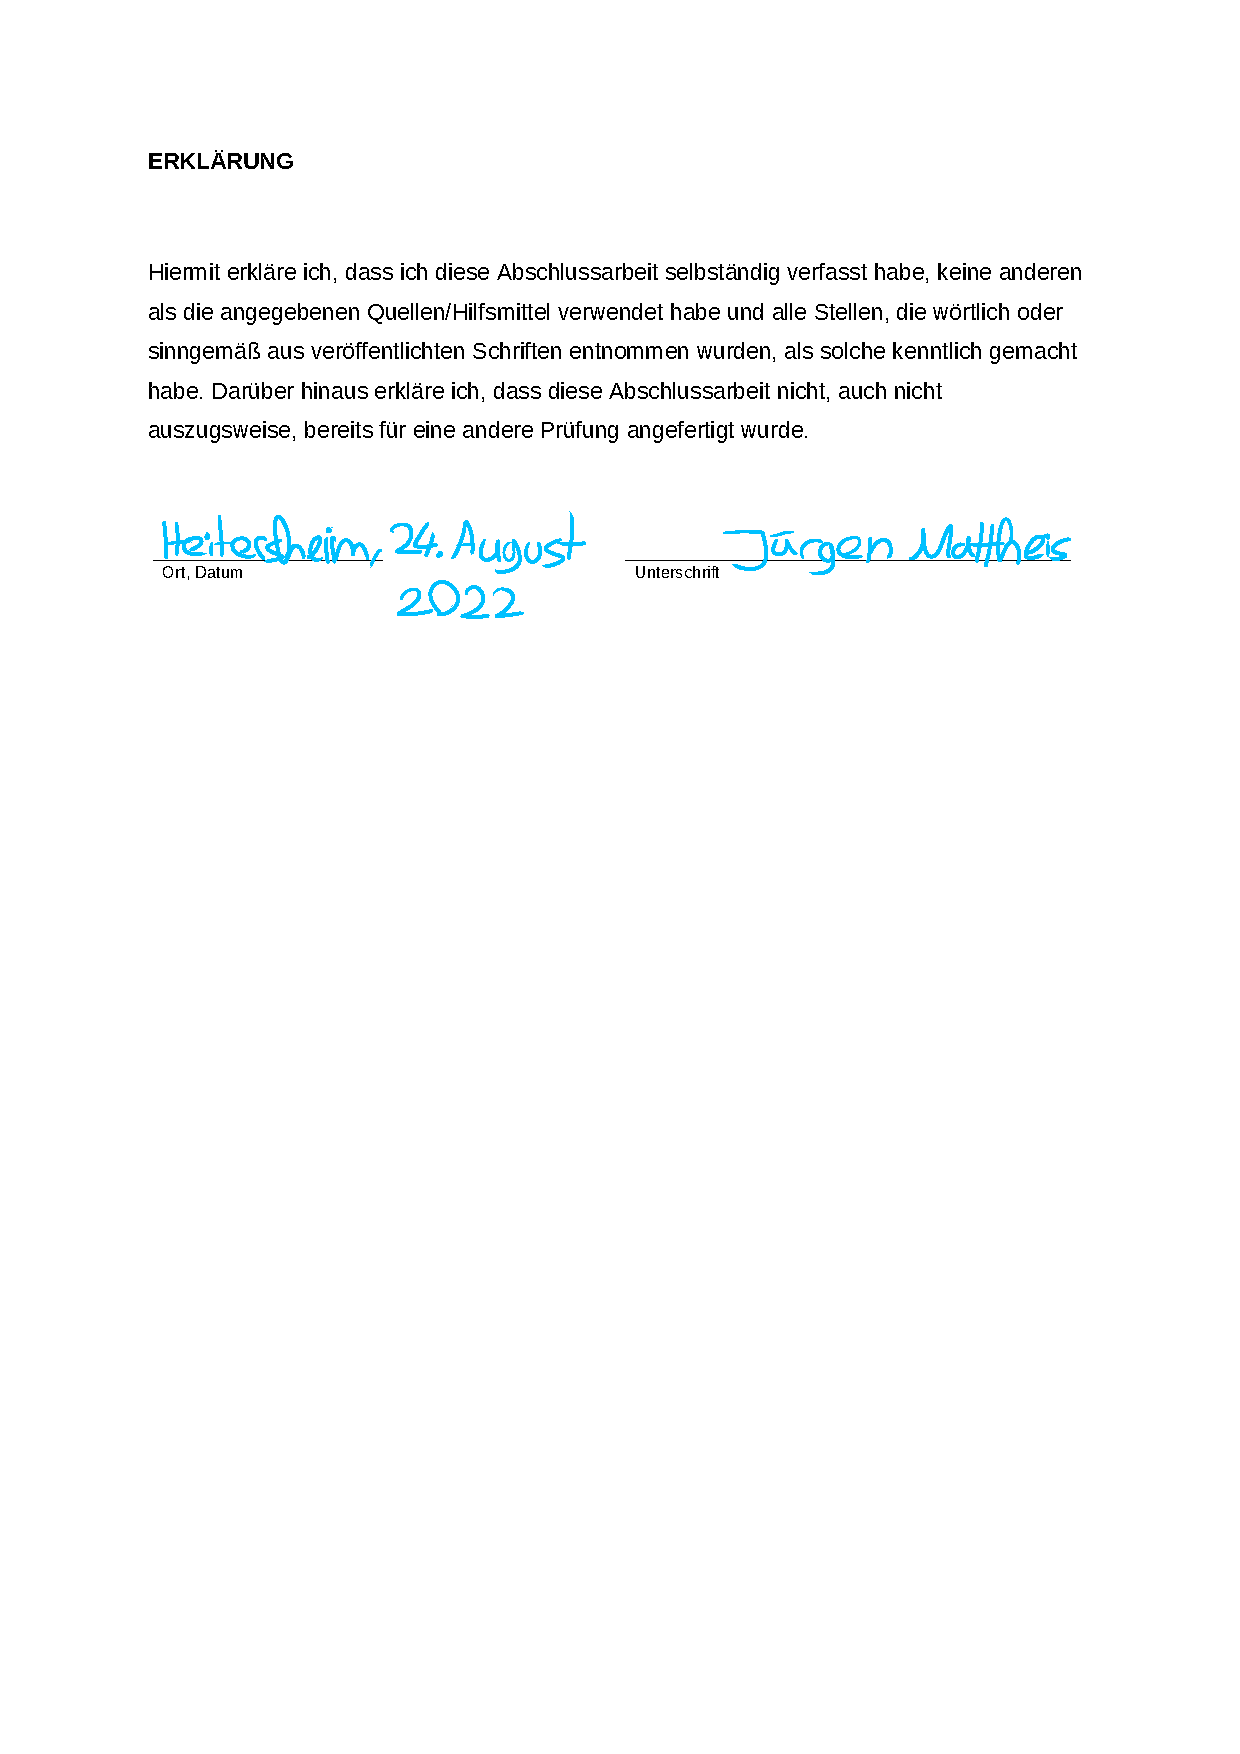
\includepdf[pages=-]{./ErklrungfrdieAbschlussarbeit_unterschrieben.pdf}

  \tableofcontents
  \listoffigures
  \listofcodecaptions
  \listoftables
  % https://tex.stackexchange.com/questions/538528/tcolorbox-newtcbtheorem-index-with-tcolorbox
  \tcblistof[\chapter*]{theorem_list}{Definitionsverzeichnis}
  % https://tex.stackexchange.com/questions/49155/how-can-i-list-items-created-with-the-float-package-in-the-toc
  \listof{floatgrammar}{Grammatikverzeichnis}

  \newtcbtheorem[list inside={theorem_list},crefname={definition}{definitions}, number within=chapter]{Definition}{Definition}%
  {enhanced, arc=0mm,top=3mm,bottom=3mm, boxrule=0mm, borderline south={1mm}{0pt}{PrimaryColor}, title style={color=PrimaryColor},
  interior style={opacity=0.2, fill=PrimaryColor},
  frame style={color=white}, fonttitle=\bfseries, fontupper=\itshape,
  before upper=\setlength{\parskip}{1em}
  }{def}

  \newtcolorbox{Special_Paragraph}{enhanced, breakable, sharpish corners, notitle, arc=0mm, left=3mm, right=3mm, boxrule=1mm, borderline vertical={1mm}{0pt}{PrimaryColor},
  interior style={fill=SecondaryColor},
  frame style={color=white},
  % https://tex.stackexchange.com/questions/459870/paragraph-breaks-inside-tcolorbox, maybe also parbox=false
  before upper=\setlength{\parskip}{1em}
  }

  % https://tex.stackexchange.com/questions/319355/tcolorbox-breakable-option-not-working
  \newtcbinputlisting{\codebox}[2][]{
  listing file={#2},
  enhanced, colframe=PrimaryColor,colback=SecondaryColor, fonttitle=\bfseries, arc=0mm, #1, listing only, listing engine=minted, minted style=colorful, minted options={fontsize=\small,breaklines,autogobble}, halign title=center, sharpish corners, drop fuzzy shadow, minted options={linenos=false, numbersep=0mm}
  }
% drop fuzzy shadow, drop lifted shadow, listing engine=listings


  \newtcbinputlisting{\numberedcodebox}[2][]{
  listing file={#2},
  enhanced, breakable, colframe=PrimaryColor,colback=white, fonttitle=\bfseries, arc=0mm, #1, listing only, listing engine=minted, minted style=colorful, halign title=center, sharpish corners, drop fuzzy shadow, overlay={\begin{tcbclipinterior}\fill[PrimaryColor] (frame.south west) rectangle ([xshift=5mm]frame.north west);\end{tcbclipinterior}}
  }

  % \newtcbinputlisting{\treebox}[2][]{
  % listing file={#2},
  % enhanced, colframe=PrimaryColor, colback=SecondaryColor, fonttitle=\bfseries, arc=0mm, #1, listing only, , halign title=center, sharpish corners, drop fuzzy shadow
  % }

  %!Tex Root = ../Main.tex
% ./Packete_und_Deklarationen.tex
\chapter{Motivation}
\label{ch:motivation}

\section{PicoC und RETI}
\section{Aufgabenstellung}
% erweitern des Compilers aus dem Bachelorprojekt
\section{Eigenheiten der Sprache C}
% Abhängigkeit von Typ von Variable usw.
% Designfehler
% Spiral Rule
% Specifier, die ganzen Begriffe aus calcourse
\section{Richtlinien}
% Email an Scholl
% exakt gleiche Präzidenzregeln
% kein unnötiger Schnickschnack
              % ./content/Motivation.tex
  \include{./content/Einführung}              % ./content/Einführung.tex
  %!Tex Root = ../Main.tex
% ./Packete_und_Deklarationen.tex
% ./Titlepage.tex
% ./Motivation.tex
% ./Einführung.tex
% ./Implementierung2.tex
% ./Ergebnisse_und_Ausblick.tex

\chapter{Implementierung}
\label{ch:implementierung}

\section{Lexikalische Analyse}
\subsection{Konkrette Syntax für die Lexikalische Analyse}
\numberwithin{floatgrammar}{section}

\label{sec:lex_analyse_verwendung_von_lark}
% ./concrete_syntax_picoc.lark
\begin{grammar}[Konkrette Syntax für die Lexikalische Analyse in EBNF, Teil 1][H][gr:concrete_syntax_lex_teil_1]
  \toprule
  \firstcase{COMMENT}{\dq //\dq\enspace /[{\wedge}\backslash n]{*}/\gralt \dq {/*}\dq\enspace  /(.\mid \setminus n)*?/\enspace \dq {*/}\dq }{L\_Comment}
  \firstcase{RETI\_COMMENT.2}{\dq {//}\dq \dq \text{\textvisiblespace} \dq ? \dq \#\dq /[\wedge\backslash n]{*}/}{}
  \midrule
  \firstcase{DIG\_NO\_0}{\dq 1\dq \gralt \dq 2\dq \gralt \dq 3\dq \gralt \dq 4\dq \gralt \dq 5\dq}{L\_Arith}
  \otherform{\dq 6\dq \gralt \dq 7\dq \gralt \dq 8\dq \gralt \dq 9\dq}{}
  \firstcase{DIG\_WITH\_0}{\dq 0\dq \gralt DIG\_NO\_0}{}
  \firstcase{NUM}{\dq 0\dq \gralt DIG\_NO\_0 DIG\_WITH\_0*}{}
  \firstcase{ASCII\_CHAR}{\dq\text{\textvisiblespace} \dq ..\dq \sim\dq }{}
  \firstcase{CHAR}{\dq '\dq ASCII\_CHAR\dq '\dq }{}
  \firstcase{FILENAME}{ASCII\_CHAR+\dq .picoc\dq }{}
  \firstcase{LETTER}{\dq {a}\dq ..\dq {z}\dq \gralt \dq {A}\dq ..\dq {Z}\dq}{}
  \firstcase{NAME}{(LETTER\gralt \dq \_\dq )}{}
  & & \qquad(LETTER\gralt DIG\_WITH\_0\gralt \dq \_\dq )* & \\
  \firstcase{name}{NAME\gralt INT\_NAME\gralt CHAR\_NAME}{}
  \otherform{VOID\_NAME}{}
  \firstcase{NOT}{\dq \sim\dq }{}
  \firstcase{REF\_AND}{\dq \&\dq }{}
  \firstcase{un\_op}{SUB\_MINUS\gralt LOGIC\_NOT\gralt NOT}{}
  \otherform{MUL\_DEREF\_PNTR \gralt REF\_AND}{}
  \firstcase{MUL\_DEREF\_PNTR}{\dq {*}\dq }{}
  \firstcase{DIV}{\dq /\dq }{}
  \firstcase{MOD}{\dq \%\dq }{}
  \firstcase{prec1\_op}{MUL\_DEREF\_PNTR\gralt DIV\gralt MOD}{}
  \firstcase{ADD}{\dq {+}\dq }{}
  \firstcase{SUB\_MINUS}{\dq {-}\dq }{}
  \firstcase{prec2\_op}{ADD\gralt SUB\_MINUS}{}
  \midrule
  \firstcase{LT}{\dq {<}\dq }{L\_Logic}
  \firstcase{LTE}{\dq {<=}\dq }{}
  \firstcase{GT}{\dq {>}\dq }{}
  \firstcase{GTE}{\dq {>=}\dq }{}
  \firstcase{rel\_op}{LT\gralt LTE\gralt GT\gralt GTE}{}
  \firstcase{EQ}{\dq {==}\dq }{}
  \firstcase{NEQ}{\dq {!=}\dq }{}
  \firstcase{eq\_op}{EQ\gralt NEQ}{}
  \firstcase{LOGIC\_NOT}{\dq !\dq }{}
  \bottomrule
\end{grammar}

\begin{grammar}[Konkrette Syntax für die Lexikalische Analyse in EBNF, Teil 2][H][gr:concrete_syntax_lex_teil_2]
  \toprule
  \firstcase{INT\_DT.2}{\dq int\dq }{L\_Assign\_Alloc}
  \firstcase{INT\_NAME.3}{\dq int\dq\enspace (LETTER\gralt DIG\_WITH\_0\gralt \dq \_\dq )+}{}
  \firstcase{CHAR\_DT.2}{\dq char\dq }{}
  \firstcase{CHAR\_NAME.3}{\dq char\dq\enspace (LETTER\gralt DIG\_WITH\_0\gralt \dq \_\dq )+}{}
  \firstcase{VOID\_DT.2}{\dq void\dq }{}
  \firstcase{VOID\_NAME.3}{\dq void\dq\enspace (LETTER\gralt DIG\_WITH\_0\gralt \dq \_\dq )+}{}
  \firstcase{prim\_dt}{INT\_DT\gralt CHAR\_DT\gralt VOID\_DT}{}
  \bottomrule
\end{grammar}

% \begin{grammar}[\(\lambda\) calculus syntax][p][gr:ex1]
%   \firstcase{T}{\nonterm{V}}{Variable}
%   \otherform{(\nonterm{T}\ \nonterm{T})}{Application}
%   \otherform{\lambda \nonterm{V}\cdot\nonterm{T}}{Abstraction}
%   \firstcase{V}{x, y, \dots}{Variables}
% \end{grammar}
% \begin{grammar}[Advanced capabilities of \texttt{grammar.sty}][p][gr:ex2]
%   \firstcase{A}{\nonterm{T} \gralt \nonterm{V}}{Multiple option on a single line}
%   \highlight
%   \otherform{\nonterm{A}}{Highlighted form}
%   \downplay
%   \otherform{\nonterm{B}\gralt \nonterm{C}}{Downplayed form}
%   \otherform{\lochighlight{\nonterm{A}} \gralt \nonterm{B}}{Emphasize part of the line}
% \end{grammar}

% erwähnen, dass in Lark die Grammatiken L_Lex und L_Parse gemischt sind
% EBNF erwähnen
% (erwähnen, dass finalle Grammatik im Appendix)
\subsection{Basic Lexer}
\section{Syntaktische Analyse}
\subsection{Konkrette Syntax für die Syntaktische Analyse}
% ./concrete_syntax_picoc.lark
% https://tex.stackexchange.com/questions/851/removing-spaces-between-words-in-math-mode
In \ref{gr:concrete_syntax_parser}

\begin{grammar}[Konkrette Syntax Syntaktische Analyse in EBNF, Teil 1][H][gr:concrete_syntax_parser]
  \toprule
	\downplay
  \firstcase{prim\_exp}{name\gralt NUM\gralt CHAR\gralt "("logic\_or")"}{L\_Arith +}
	\downplay
  \firstcase{post\_exp}{array\_subscr\gralt struct\_attr\gralt fun\_call}{L\_Array +}
	\downplay
  \otherform{input\_exp\gralt print\_exp\gralt prim\_exp}{L\_Pntr +}
	\downplay
  \firstcase{un\_exp}{un\_op un\_exp\gralt post\_exp}{L\_Struct + L\_Fun}
  \midrule
	\downplay
  \firstcase{input\_exp}{\dq input\dq\dq(\dq\dq)\dq}{L\_Arith}
	\downplay
  \firstcase{print\_exp}{\dq print\dq\dq(\dq logic\_or\dq)\dq}{}
	\downplay
  \firstcase{arith\_prec1}{arith\_prec1\enspace prec1\_op\enspace un\_exp\gralt un\_exp}{}
	\downplay
  \firstcase{arith\_prec2}{arith\_prec2\enspace prec2\_op\enspace arith\_prec1\gralt arith\_prec1}{}
	\downplay
  \firstcase{arith\_and}{arith\_and\enspace \dq\&\dq\enspace arith\_prec2\gralt arith\_prec2}{}
	\downplay
  \firstcase{arith\_oplus}{arith\_oplus\enspace \dq {\wedge{}}\dq\enspace arith\_and\gralt arith\_and}{}
	\downplay
  \firstcase{arith\_or}{arith\_or\enspace \dq{\mid} \dq\enspace arith\_oplus\gralt arith\_oplus}{}
  \midrule
  \downplay
  \firstcase{rel\_exp}{rel\_exp\enspace rel\_op\enspace arith\_or\gralt arith\_or}{L\_Logic}
  \downplay
  \firstcase{eq\_exp}{eq\_exp\enspace eq\_op rel\_exp\gralt rel\_exp}{}
  \downplay
  \firstcase{logic\_and}{logic\_and\enspace \dq{\&\&}\dq\enspace eq\_exp\gralt eq\_exp}{}
  \downplay
  \firstcase{logic\_or}{logic\_or\enspace \dq{\mid\mid}\dq\enspace logic\_and\gralt logic\_and}{}
  \midrule
	\downplay
  \firstcase{type\_spec}{prim\_dt\gralt struct\_spec}{L\_Assign\_Alloc}
	\downplay
  \firstcase{alloc}{type\_spec\enspace pntr\_decl}{}
	\downplay
  \firstcase{assign\_stmt}{un\_exp\enspace \dq {=}\dq\enspace logic\_or\dq ;\dq }{}
  \firstcase{initializer}{logic\_or\gralt array\_init\gralt struct\_init}{}
	\downplay
  \firstcase{init\_stmt}{alloc\enspace \dq {=}\dq\enspace initializer\dq ;\dq }{}
	\downplay
  \firstcase{const\_init\_stmt}{\dq const\dq\enspace type\_spec\enspace name\enspace \dq {=}\dq\enspace NUM\dq ;\dq }{}
  \midrule
  \firstcase{pntr\_deg}{\dq {*}\dq *}{L\_Pntr}
  \firstcase{pntr\_decl}{pntr\_deg\enspace array\_decl\gralt array\_decl}{}
  \midrule
  \firstcase{array\_dims}{(\dq [\dq NUM\dq ]\dq )*}{L\_Array}
  \firstcase{array\_decl}{name\enspace array\_dims\gralt \dq (\dq pntr\_decl\dq )\dq  array\_dims}{}
  \firstcase{array\_init}{\dq \{\dq initializer(\dq ,\dq\enspace initializer)*\dq \}\dq }{}
  \firstcase{array\_subscr}{post\_exp\dq [\dq logic\_or\dq ]\dq }{}
  \midrule
  \firstcase{struct\_spec}{\dq struct\dq\enspace name}{L\_Struct}
  \firstcase{struct\_params}{(alloc\dq ;\dq )+}{}
  \firstcase{struct\_decl}{\dq struct\dq\enspace name\enspace \dq \{\dq struct\_params\dq \}\dq }{}
  \firstcase{struct\_init}{\dq \{\dq \dq .\dq name\dq {=}\dq initializer}{}
  & & \qquad(\dq ,\dq\enspace \dq .\dq name\dq {=}\dq initializer)*\dq \}\dq & \\
  \firstcase{struct\_attr}{post\_exp\dq .\dq name}{}
  \midrule
	\downplay
  \firstcase{if\_stmt}{\dq if\dq \dq (\dq logic\_or\dq )\dq\enspace exec\_part}{L\_If\_Else}
	\downplay
  \firstcase{if\_else\_stmt}{\dq if\dq \dq (\dq logic\_or\dq )\dq\enspace exec\_part\enspace \dq else\dq\enspace exec\_part}{}
  \midrule
	\downplay
  \firstcase{while\_stmt}{\dq while\dq \dq (\dq logic\_or\dq )\dq\enspace exec\_part}{L\_Loop}
	\downplay
  \firstcase{do\_while\_stmt}{\dq do\dq\enspace exec\_part\enspace \dq while \dq \dq (\dq logic\_or\dq )\dq \dq ;\dq }{}
  \bottomrule
\end{grammar}

\begin{grammar}[Konkrette Syntax für die Syntaktische Analyse in EBNF, Teil 2][H]
  \toprule
	\downplay
  \firstcase{decl\_exp\_stmt}{alloc\dq ;\dq }{L\_Stmt}
	\downplay
  \firstcase{decl\_direct\_stmt}{ assign\_stmt\gralt init\_stmt\gralt const\_init\_stmt}{}
  \firstcase{decl\_part}{ decl\_exp\_stmt\gralt decl\_direct\_stmt\gralt RETI\_COMMENT}{}
  \\[-0.2cm]
	\downplay
  \firstcase{compound\_stmt}{ \dq \{\dq exec\_part* \dq \}\dq }{}
	\downplay
  \firstcase{exec\_exp\_stmt}{logic\_or\dq ;\dq }{}
	\downplay
  \firstcase{exec\_direct\_stmt}{if\_stmt\gralt if\_else\_stmt\gralt while\_stmt\gralt do\_while\_stmt}{}
	\downplay
  \otherform{assign\_stmt\gralt fun\_return\_stmt}{}
  \firstcase{exec\_part}{compound\_stmt\gralt exec\_exp\_stmt\gralt exec\_direct\_stmt}{}
  \otherform{RETI\_COMMENT}{}
  \\[-0.2cm]
  \firstcase{decl\_exec\_stmts}{decl\_part* exec\_part*}{}
  \midrule
  \firstcase{fun\_args}{[logic\_or(\dq ,\dq\enspace logic\_or)*]}{L\_Fun}
  \firstcase{fun\_call}{name\dq (\dq fun\_args\dq )\dq }{}
  \firstcase{fun\_return\_stmt}{\dq return\dq\enspace [logic\_or]\dq ;\dq }{}
  \firstcase{fun\_params}{[alloc(\dq ,\dq\enspace alloc)*]}{}
  \firstcase{fun\_decl}{type\_spec\enspace pntr\_deg\enspace name\dq (\dq fun\_params\dq )\dq }{}
  \firstcase{fun\_def}{type\_spec\enspace pntr\_deg\enspace name\dq (\dq fun\_params\dq )\dq\enspace \dq \{\dq  decl\_exec\_stmts \dq \}\dq }{}
  \midrule
  \firstcase{decl\_def}{(struct\_decl\gralt fun\_decl)\dq ;\dq \gralt fun\_def}{L\_File}
  \firstcase{decls\_defs}{decl\_def*}{}
  \firstcase{file}{FILENAME\enspace decls\_defs}{}
  \bottomrule
\end{grammar}
% Vorteile von Lark
\subsection{Umsetzung von Präzidenz}
Die \colorbold{PicoC} Programmiersprache hat dieselben \colorbold{Präzidenzregeln} implementiert, wie die Programmiersprache \colorbold{C} \footcite{noauthor_c_nodate}. Die \colorbold{Präzidenzregeln} von \colorbold{PicoC} sind in Tabelle~\ref{tab:reference_table} aufgelistet.

% \rowcolors{2}{SecondaryColor}{white}
\begin{table}[H]
  \center
  % \Block{2}{=}{Links, dann rechts $\rightarrow$} \\
  \begin{NiceTabular}{X[1,c]X[2,c]X[3,l]X[2,c]}[rules/color=PrimaryColor] % {\linewidth}{|C|C|L|L|}
  \CodeBefore
  \rowcolor{PrimaryColor}{1}
  \rowcolors{2-18}{SecondaryColor}{}[cols={2-3}]
  \rowcolors{2-18}{SecondaryColor}{}[cols={1,4}, respect-blocks, restart]
  \Body
  \textbf{\textcolor{white}{Präzidenz}} &	\textbf{\textcolor{white}{Operator}} & \textbf{\textcolor{white}{Beschreibung}} &	\textbf{\textcolor{white}{Assoziativität}} \\
  1	& \verb|a()|	& Funktionsaufruf & \Block{3-1}{Links, dann rechts $\rightarrow$} \\
    & \verb|a[]|	& Indexzugriff & \\
    & \verb|a.b| & Attributzugriff & \\
  2	&	\verb|-a| & Unäres Minus & \Block{3-1}{Rechts, dann links $\leftarrow$} \\
    & \smalltt{!a $\thicksim$a}	& Logisches NOT und Bitweise NOT & \\
    & \verb|*a &a| & Dereferenz und Referenz, auch Adresse-von & \\
  3	& \smalltt{a*b a/b a\%b} &	Multiplikation, Division und Modulo & \Block{9-1}{Links, dann rechts $\rightarrow$} \\
  4	& \verb|a+b a-b|	& Addition und Subtraktion & \\
  5	& \verb|a<b a<=b| \verb|a>b a>=b| & Kleiner, Kleiner Gleich, Größer, Größer gleich & \\
  6 &	\verb|a==b a!=b| & Gleichheit und Ungleichheit & \\
  7 &	\verb|a&b| & Bitweise UND & \\
  8 &	\verb|a^b| & Bitweise XOR (exclusive or) & \\
  9 & \smalltt{a$\mid$b} & Bitweise ODER (inclusive or) & \\
  10	& \verb|a&&b| &	Logiches UND & \\
  11	& $a{\mid\mid} b$	& Logisches ODER & \\
  12 & \verb|a=b| & Zuweisung & Rechts, dann links $\leftarrow$ \\
  13 &	\verb|a,b|& Komma	& Links, dann rechts $\rightarrow$ \\
  \bottomrule
\end{NiceTabular}
\caption{Präzidenzregeln von PicoC}
\label{tab:reference_table}
\end{table}
% erwähnen von Mehrdeutigkeit und Assoziativität
% finalle Grammatik im Appendix
% Crafting Compilers Quelle benennen

\subsection{Derivation Tree Generierung}
\subsubsection{Early Parser}
\subsubsection{Codebeispiel}
\label{sec:derivation_tree_generierung}
\begin{code}
  \centering
  \numberedcodebox[minted language=c]{./code_examples/example_dt_simple_ast_gen_array_decl_and_alloc.picoc}
  \caption{PicoC Code für Derivation Tree Generierung}
  \label{code:picoc_code_für_derivation_tree_generierung}
\end{code}

\begin{code}
  \centering
  \numberedcodebox[minted language=text]{./code_examples/example_dt_simple_ast_gen_array_decl_and_alloc.dt}
  \caption{Derivation Tree nach Derivation Tree Generierung}
  \label{code:derivation_tree_nach_derivation_tree_generierung}
\end{code}

\subsection{Derivation Tree Vereinfachung}
\subsubsection{Visitor}
\subsubsection{Codebeispiel}

Beispiel aus Subkapitel~\ref{sec:derivation_tree_generierung} wird fortgeführt.

\begin{code}
  \centering
  \numberedcodebox[minted language=text]{./code_examples/example_dt_simple_ast_gen_array_decl_and_alloc.dt_simple}
  \caption{Derivation Tree nach Derivation Tree Vereinfachung}
  \label{code:picoc_code_nach_derivation_tree_vereinfachung}
\end{code}

% Visitor erwähnen
\subsection{Abstrakt Syntax Tree Generierung}
\subsubsection{PicoC-Knoten}
% Tabelle aller PicoC Knoten
% möglichst kurze und leicht verständliche Bezeichner für Knoten

\begin{table}[H]
  \center
  \begin{NiceTabular}{X[7]X[10]}[rules/color=PrimaryColor]
  \CodeBefore
  \rowcolor{PrimaryColor}{1}
  \rowcolors{2-17}{SecondaryColor}{}[cols={1-2}]
  \Body
  \textbf{\textcolor{white}{PiocC-Knoten}} & \textbf{\textcolor{white}{Beschreibung}} \\
  \smalltt{Name(val)} & Ein \colorbold{Bezeichner}, z.B. \smalltt{my\_fun, my\_var} usw. , aber da es keine gute Kurzform für \smalltt{Identifier()} (englisches Wort für Bezeichner) gibt, wurde dieser Knoten \smalltt{Name()} genannt. \\
  \smalltt{Num(val)} & Eine \colorbold{Zahl}, z.B. \smalltt{42, -3} usw. \\
  \smalltt{Char(val)} & Ein \colorbold{Zeichen} der \colorbold{ASCII-Zeichenkodierung}, z.B. \smalltt{'c', '*'} usw. \\
  \smalltt{Minus(), Not(), DerefOp(), RefOp(), LogicNot()} & Die \colorbold{unären Operatoren} \smalltt{un\_op}: \smalltt{-a, {$\thicksim$}a, *a, \&a !a}. \\
  \smalltt{Add(), Sub(), Mul(), Div(), Mod(), Oplus(), And(), Or(), LogicAnd(), LogicOr()} & Die \colorbold{binären Operatoren} \smalltt{bin\_op}: \smalltt{a + b, a - b, a * b, a / b, a \% b, a $\wedge$ b, a \& b, a $\mid$ b, a \&\& b, a {$\mid\mid$} b}. \\
  \smalltt{Eq(), NEq(), Lt(), LtE(), Gt(), GtE()} & Die \colorbold{Relationen} \smalltt{rel}: \smalltt{a == b, a != b, a < b, a <= b, a > b, a >= b}. \\
  \smalltt{Const(), Writeable()} & Die \colorbold{Type Qualifier} \smalltt{type\_qual}: \smalltt{const}, was für ein \colorbold{nicht beschreibbare} \colorbold{Konstante} steht und das \colorbold{nicht} Angeben von \smalltt{const}, was für einen \colorbold{beschreibbare} Variable steht. \\
\smalltt{IntType(), CharType(), VoidType()} & Die \colorbold{Type Specifier} für \colorbold{Primitiven Datentypen}, die in der Abstrakten Syntax, um eine intuitive Bezeichnung zu haben einfach nur unter \colorbold{Datentypen} \smalltt{datatype} eingeordnet werden: \smalltt{int},  \smalltt{char},  \smalltt{void}. \\
\smalltt{Placeholder()} & \colorbold{Platzhalter} für einen Knoten, der diesen später \colorbold{ersetzt}. \\
  \smalltt{BinOp(exp, bin\_op, exp)} & Container für eine \colorbold{binäre Operation} mit $2$ Expressions: \smalltt{<exp1> <bin\_op> <exp2>}\\
  \smalltt{UnOp(un\_op, exp)} & Container für eine \colorbold{unäre Operation} mit einer Expression: \smalltt{<un\_op> <exp>}. \\
  \smalltt{Exit(num)} & Container für einen \colorbold{Exit Code}, der vor der Beendigung in das \smalltt{ACC} Register geschrieben wird und steht für die \colorbold{Beendigung} des laufenden Programmes. \\
  \smalltt{Atom(exp, rel, exp)} & Container für eine \colorbold{binäre Relation} mit $2$ Expressions: \smalltt{<exp1> <rel> <exp2>}\\
  \smalltt{ToBool(exp)} & Container für einen \colorbold{Arithmetischen Ausdruck}, wie z.B. \smalltt{1 + 3} oder einfach nur \smalltt{3}, der nicht nur $1$ oder $0$ als Ergebnis haben kann und daher bei einem Ergebnis $x > 1$ auf $1$ abgebildet wird. \\
  \smalltt{Alloc(type\_qual, datatype, name, \textcolor{gray!90!black}{local\_var\_or\_param})} & \colorbold{Container} für eine \colorbold{Allokation} \smalltt{<type\_qual> <datatype> <name>} mit den notwendigen Knoten \smalltt{type\_qual},  \smalltt{datatype} und  \smalltt{name}, die alle für einen Eintrag in der  \colorbold{Symboltabelle} notwendigen Informationen enthalten. Zudem besitzt er ein \textcolor{gray!90!black}{verstecktes Attribut}  \smalltt{local\_var\_or\_param}, dass die Information trägt, ob es sich bei der \colorbold{Variable} um eine \colorbold{Lokale Variable} oder einen \colorbold{Parameter} handelt. \\
  \smalltt{Assign(lhs, exp)} & Container für eine \colorbold{Zuweisung}, wobei \smalltt{lhs} ein  \smalltt{Subscr(exp1, exp2)}, \smalltt{Deref(exp1, exp2)}, \smalltt{Attr(exp, name)} oder  \smalltt{Name('var')} sein kann und  \smalltt{exp} ein beliebiger \colorbold{Logischer Ausdruck} sein kann: \smalltt{lhs = exp}. \\
  \bottomrule
\end{NiceTabular}
\caption{PicoC-Knoten Teil 1}
\label{tab:picoc_knoten_teil_1}
\end{table}

\begin{table}[H]
  \center
  \begin{NiceTabular}{X[7]X[10]}[rules/color=PrimaryColor]
  \CodeBefore
  \rowcolor{PrimaryColor}{1}
  \rowcolors{2-13}{SecondaryColor}{}[cols={1-2}]
  \Body
  \textbf{\textcolor{white}{PiocC-Knoten}} & \textbf{\textcolor{white}{Beschreibung}} \\
  \smalltt{Exp(exp, \textcolor{gray!90!black}{datatype}, \textcolor{gray!90!black}{error\_data})} & Container für einen \colorbold{beliebigen Ausdruck}, dessen Ergebnis auf den \colorbold{Stack} soll. Zudem besitzt er $2$ \textcolor{gray!90!black}{versteckte Attribute}, wobei \smalltt{datatype} im \colorbold{RETI Blocks Pass} wichtig ist und \smalltt{error\_data} für \colorbold{Fehlermeldungen} wichtig ist. \\
  \smalltt{Stack(num)} & Container, der für das \colorbold{temporäre} Ergebnis einer Berechnung, das \smalltt{num} Speicherzellen relativ zum  \colorbold{Stackpointer Register} \smalltt{SP} steht.\\
  \smalltt{Stackframe(num)} & Container, der für eine Variable steht, die \smalltt{num} Speicherzellen relativ zum \colorbold{Begin-Aktive-Funktion Register} \smalltt{BAF} steht. \\
  \smalltt{Global(num)} & Container, der für eine Variable steht, die \smalltt{num} Speicherzellen relativ zum \colorbold{Datensegment Register} \smalltt{DS} steht. \\
  \smalltt{StackMalloc(num)} & Container, der für das \colorbold{Allokieren} von \smalltt{num} Speicherzellen auf dem \colorbold{Stack} steht. \\
\smalltt{PntrDecl(num, datatype)} & Container, der für den \colorbold{Pointerdatentyp} steht: \smalltt{<prim\_dt> *<var>}, wobei das \colorbold{Attribut} \smalltt{num} die \colorbold{Anzahl zusammengefasster Pointer} angibt und \smalltt{datatype} der {Datentyp} ist, auf den der oder die \colorbold{Pointer} zeigen. \\
\smalltt{Ref(exp, \textcolor{gray!90!black}{datatype}, \textcolor{gray!90!black}{error\_data})} & Container, der für die Anwendung des \colorbold{Referenz-Operators} \smalltt{\&<var>} steht und die \colorbold{Adresse} einer \colorbold{Location} auf den Stack schreiben soll, die über \smalltt{exp} eingegrenzt wird. Zudem besitzt er $2$ \textcolor{gray!90!black}{versteckte Attribute}, wobei \smalltt{datatype} im \colorbold{RETI Blocks Pass} wichtig ist und \smalltt{error\_data} für \colorbold{Fehlermeldungen} wichtig ist. \\
\smalltt{Deref(lhs, exp)} & Container für den \colorbold{Indexzugriff} auf einen \colorbold{Array-} oder \colorbold{Pointerdatentyp}: \smalltt{<var>[<i>]}, wobei \smalltt{exp1} eine angehängte weitere \smalltt{Subscr(exp1, exp2)}, \smalltt{Deref(exp1, exp2)}, \smalltt{Attr(exp, name)} oder ein \smalltt{Name('var')} sein kann und \smalltt{exp2} der Index ist auf den zugegriffen werden soll. \\
\smalltt{ArrayDecl(nums, datatype)} & Container, der für den \colorbold{Arraydatentyp} steht: \smalltt{<prim\_dt> <var>[<i>]}, wobei das \colorbold{Attribut} \smalltt{nums} eine Liste von \smalltt{Num('x')} ist, die die \colorbold{Dimensionen} des Arrays angibt und \smalltt{datatype} der {Datentyp} ist, der über das Anwenden von \smalltt{Subscript()} auf das Array zugreifbar ist. \\
\smalltt{Array(exps, \textcolor{gray!90!black}{datatype})} & Container für den \colorbold{Initializer} eines \colorbold{Arrays}, dessen Einträge \smalltt{exps} weitere Initializer für eine \colorbold{Array-Dimension} oder ein Initializer für ein \colorbold{Struct} oder ein \colorbold{Logischer Ausdruck} sein können, z.B. \smalltt{\{\{1, 2\}, \{3, 4\}\}}. Des Weiteren besitzt er ein \textcolor{gray!90!black}{verstecktes Attribut} \smalltt{datatype}, welches für den \colorbold{PicoC-Mon Pass} Informationen transportiert, die für \colorbold{Fehlermeldungen} wichtig sind. \\
\smalltt{Subscr(exp1, exp2)} & Container für den \colorbold{Indexzugriff} auf einen \colorbold{Array-} oder \colorbold{Pointerdatentyp}: \smalltt{<var>[<i>]}, wobei \smalltt{exp1} eine angehängte weitere \smalltt{Subscr(exp1, exp2)}, \smalltt{Deref(exp1, exp2)} oder \smalltt{Attr(exp, name)} Operation sein kann oder ein \smalltt{Name('var')} sein kann und \smalltt{exp2} der Index ist auf den zugegriffen werden soll. \\
  \smalltt{StructSpec(name)} & Container für einen selbst definierten \colorbold{Structdatentyp}: \smalltt{struct <name>}, wobei das \colorbold{Attribut} \smalltt{name} festlegt, welchen \colorbold{selbst definierte} Structdatentyp dieser Container-Knoten repräsentiert. \\
  \smalltt{Attr(exp, name)} & Container für den \colorbold{Attributzugriff} auf einen \colorbold{Structdatentyp}: \smalltt{<var>.<attr>}, wobei \smalltt{exp1} eine angehängte weitere \smalltt{Subscr(exp1, exp2)}, \smalltt{Deref(exp1, exp2)} oder \smalltt{Attr(exp, name)} Operation sein kann oder ein \smalltt{Name('var')} sein kann und \smalltt{name} das Attribut ist, auf das zugegriffen werden soll. \\
  \bottomrule
\end{NiceTabular}
\caption{PicoC-Knoten Teil 2}
\label{tab:picoc_knoten_teil_2}
\end{table}

\begin{table}[H]
  \center
  \begin{NiceTabular}{X[7]X[10]}[rules/color=PrimaryColor]
  \CodeBefore
  \rowcolor{PrimaryColor}{1}
  \rowcolors{2-9}{SecondaryColor}{}[cols={1-2}]
  \Body
  \textbf{\textcolor{white}{PiocC-Knoten}} & \textbf{\textcolor{white}{Beschreibung}} \\
  \smalltt{Struct(assigns, \textcolor{gray!90!black}{datatype})} & Container für den \colorbold{Initializer} eines \colorbold{Structs}, z.B \smalltt{\{.<attr1>=\{1, 2\}, .<attr2>=\{3, 4\}\}}, dessen Eintrag \smalltt{assigns} eine Liste von \smalltt{Assign(lhs, exp)} ist mit einer Zuordnung eines \colorbold{Attributezeichners}, zu einem weiteren Initializer für eine \colorbold{Array-Dimension} oder zu einem Initializer für ein \colorbold{Struct} oder zu einem \colorbold{Logischen Ausdruck}. Des Weiteren besitzt er ein  \textcolor{gray!90!black}{verstecktes Attribut} \smalltt{datatype}, welches für den \colorbold{PicoC-Mon Pass} Informationen transportiert, die für \colorbold{Fehlermeldungen} wichtig sind. \\
  \smalltt{StructDecl(name, allocs)} & Container für die Deklaration eines \colorbold{selbstdefinierten Structdatentyps}, z.B. \smalltt{struct <var> \{<datatype> <attr1>; <datatype> <attr2>;\};}, wobei \smalltt{name} der \colorbold{Bezeichner} des Structdatentyps ist und \smalltt{allocs} eine Liste von Bezeichnern der \colorbold{Attribute} des Structdatentyps mit dazugehörigem \colorbold{Datentyp}, wofür sich der \colorbold{Container-Knoten} \smalltt{Alloc(type\_qual, datatype, name)} sehr gut als \colorbold{Container} eignet. \\
  \smalltt{If(exp, stmts\_goto)} & Container für ein \colorbold{If Statement} \smalltt{if(<exp>) \{ <stmts> \}} inklusive  \colorbold{Condition}  \smalltt{exp} und einem  \colorbold{Branch}  \smalltt{stmts\_goto}, indem eine \colorbold{Liste von Statements} stehen kann oder ein einzelnes \smalltt{GoTo(Name('block.xyz'))}. \\
  \smalltt{IfElse(exp, stmts\_goto1, stmts\_goto2)} & Container für ein \colorbold{If-Else Statement} \smalltt{if(<exp>) \{ <stmts2> \} else \{ <stmts2> \}} inklusive \colorbold{Codition} \smalltt{exp} und $2$ \colorbold{Branches} \smalltt{stmts\_goto1} und \smalltt{stmts\_goto2}, die zwei Alternativen Darstellen in denen jeweils \colorbold{Listen von Statements} oder  \smalltt{GoTo(Name('block.xyz'))}'s stehen können. \\
  \smalltt{While(exp, stmts\_goto)} & Container für ein \colorbold{While-Statement} \smalltt{while(<exp>) \{ <stmts> \}} inklusive  \colorbold{Condition}  \smalltt{exp} und einem \colorbold{Branch}  \smalltt{stmts\_goto}, indem eine \colorbold{Liste von Statements} stehen kann oder ein einzelnes \smalltt{GoTo(Name('block.xyz'))}. \\
  \smalltt{DoWhile(exp, stmts\_goto)} & Container für ein \colorbold{Do-While-Statement} \smalltt{do \{ <stmts> \} while(<exp>);} inklusive  \colorbold{Condition}  \smalltt{exp} und einem \colorbold{Branch}  \smalltt{stmts\_goto}, indem eine \colorbold{Liste von Statements} stehen kann oder ein einzelnes \smalltt{GoTo(Name('block.xyz'))}. \\
  \smalltt{Call(name, exps)} & Container für einen \colorbold{Funktionsaufruf}: \smalltt{fun\_name(exps)}, wobei \smalltt{name} der \colorbold{Bezeichner} der Funktion ist, die aufgerufen werden soll und \smalltt{exps} eine \colorbold{Liste von Argumenten} ist, die an die Funktion übergeben werden soll. \\
  \smalltt{Return(exp)} & Container für ein \smalltt{Return-Statement}: \smalltt{return <exp>}, wobei das  \colorbold{Attribut}  \smalltt{exp} einen  \colorbold{Logischen Ausdruck} darstellt, dessen Ergebnis vom  \colorbold{Return-Statement} zurückgegeben wird. \\
  \smalltt{FunDecl(datatype, name, allocs)} & Container für eine \colorbold{Funktionsdeklaration}, z.B. \smalltt{<datatype> <fun\_name>(<datatype> <param1>, <datatype> <param2>)}, wobei \smalltt{datatype} der  \colorbold{Rückgabewert} der Funktion ist,  \smalltt{name} der  \colorbold{Bezeichner} der Funktion ist und \smalltt{allocs} die \colorbold{Parameter} der Funktion sind, wobei der \colorbold{Container-Knoten} \smalltt{Alloc(type\_spec, datatype, name)} als Cotainer für die Parameter dient. \\
  \bottomrule
\end{NiceTabular}
\caption{PicoC-Knoten Teil 3}
\label{tab:picoc_knoten_teil_3}
\end{table}

\begin{table}[H]
  \center
  \begin{NiceTabular}{X[7]X[10]}[rules/color=PrimaryColor]
  \CodeBefore
  \rowcolor{PrimaryColor}{1}
  \rowcolors{2-9}{SecondaryColor}{}[cols={1-2}]
  \Body
  \textbf{\textcolor{white}{PiocC-Knoten}} & \textbf{\textcolor{white}{Beschreibung}} \\
  \smalltt{FunDef(datatype, name, allocs, stmts\_blocks)} & Container für eine \colorbold{Funktionsdefinition}, z.B. \smalltt{<datatype> <fun\_name>(<datatype> <param>) \{<stmts>\}}, wobei \smalltt{datatype} der  \colorbold{Rückgabewert} der Funktion ist,  \smalltt{name} der  \colorbold{Bezeichner} der Funktion ist, \smalltt{allocs} die \colorbold{Parameter} der Funktion sind, wobei der \colorbold{Container-Knoten} \smalltt{Alloc(type\_spec, datatype, name)} als Cotainer für die Parameter dient und \smalltt{stmts\_blocks} eine Liste von \colorbold{Statemetns} bzw.  \colorbold{Blöcken} ist, welche diese Funktion beinhaltet. \\
  \smalltt{NewStackframe(fun\_name, goto\_after\_call)} & Container für die \colorbold{Erstellung} eines neuen \colorbold{Stackframes}, wobei \smalltt{fun\_name} der Bezeichner der Funktion ist, für die ein neuer \colorbold{Stackframe} erstellt werden soll und später dazu dient den \colorbold{Block} dieser Funktion zu finden, weil dieser für den weiteren Kompiliervorang wichtige Information in seinen \textcolor{gray!90!black}{versteckte Attribute} angehängt hat und \smalltt{goto\_after\_call} ein \smalltt{GoTo(Name('addr@next\_instr'))} ist, welches später durch die \colorbold{Adresse} der Instruction, die direkt auf die \colorbold{Jump Instruction} folgt, ersetzt wird. \\
  \smalltt{RemoveStackframe()} & Container für das \colorbold{Entfernen} des aktuellen \colorbold{Stackframes}. \\
  \smalltt{File(name, decls\_defs\_blocks)} & Container für alle \colorbold{Funkionen} oder \colorbold{Blöcke}, welche eine Datei als Ursprung haben, wobei \smalltt{name} der \colorbold{Dateiname} der Datei ist, die erstellt wird und \smalltt{decls\_defs\_blocks} eine Liste von \colorbold{Funktionen} bzw. \colorbold{Blöcken} ist. \\
  \smalltt{Block(name, stmts\_instrs, \textcolor{gray!90!black}{instrs\_before}, \textcolor{gray!90!black}{num\_instrs}, \textcolor{gray!90!black}{param\_size}, \textcolor{gray!90!black}{local\_vars\_size})} & Container für \colorbold{Statements}, der auch als \colorbold{Block} bezeichnet wird, wobei das Attribut \smalltt{name} der Bezeichners des \colorbold{Labels} des Blocks ist und \smalltt{stmts\_instrs} eine \colorbold{Liste von Statements} oder \colorbold{Instructions}. Zudem besitzt er noch $3$ \textcolor{gray!90!black}{versteckte Attribute}, wobei  \smalltt{instrs\_before} die Zahl der \colorbold{Instructions} vor diesem \colorbold{Block} zählt,  \smalltt{num\_instrs} die Zahl der Instructions ohne Kommentare in diesem Block zählt, \smalltt{param\_size} die voraussichtliche Anzahl an Speicherzellen aufaddiert, die für die \colorbold{Parameter} der Funktion belegt werden müssen und \smalltt{local\_vars\_size} die voraussichtliche Anzahl an Speicherzellen aufaddiert, die für die \colorbold{lokalen Variablen} der Funktion belegt werden müssen. \\
  \smalltt{GoTo(name)} & Container für ein \smalltt{Goto} zu einem anderen \colorbold{Block}, wobei das Attribut \smalltt{name} der Bezeichner des \colorbold{Labels} des Blocks ist zu dem Gesprungen werden soll. \\
  \smalltt{SingleLineComment(prefix, content)} & Container für einen \colorbold{Kommentar}, den der Compiler selber während des \colorbold{Kompiliervorangs} erstellt, der im \colorbold{RETI-Interpreter} selbst später \colorbold{nicht} sichtbar sein wird, aber in den \colorbold{Immediate}-Dateien, welche die \colorbold{Abstract Syntax Trees} nach den verschiedenen \colorbold{Passes} enthalten. \\
  \smalltt{RETIComment(value)} & Container für einen \colorbold{Kommentar} im Code der Form: \smalltt{// \# comment}, der im \colorbold{RETI-Intepreter} später sichtbar sein wird und zur Orientierung genutzt werden kann, allerdings in einer tatsächlichen Implementierung einer \colorbold{RETI-CPU} \colorbold{nicht umsetzbar} ist und auch nicht sinnvoll wäre umzusetzen. Der \colorbold{Kommentar} ist im Attribut \colorbold{value}, welches jeder Knoten besitzt gespeichert. \\
  \bottomrule
\end{NiceTabular}
\caption{PicoC-Knoten Teil 4}
\label{tab:picoc_knoten_teil_4}
\end{table}
\begin{Special_Paragraph}
  Die \textcolor{gray!90!black}{ausgegrauten} Attribute der PicoC-Nodes sind \textcolor{gray!90!black}{versteckte Attribute}, die \colorbold{nicht} direkt bei der Erstellung der  \colorbold{PicoC-Nodes} mit einem Wert \colorbold{initialisiert} werden, sondern im \colorbold{Verlauf der Kompilierung} beim Durchlaufen der verschiedenen Passes etwas zugewiesen bekommen, dass im weiteren Kompiliervorgang \colorbold{Informationen} transportiert, die später im Kompiliervorgang nicht mehr so leicht zugänglich wären.

  Jeder \colorbold{Knoten} hat darüberhinaus auch noch $2$ \colorbold{Attribute} \smalltt{value} und \smalltt{position}, wobei \colorbold{value} bei einem \colorbold{Token-Knoten} (Definition~\ref{def:token_knoten}) dem \colorbold{Tokenwert} des Tokens, welches es ersetzt entspricht und bei \colorbold{Container-Knoten} (Definition~\ref{def:container_knoten}) unbesetzt ist. Das \colorbold{Attribut} \smalltt{position} wird später für Fehlermeldungen gebraucht.
\end{Special_Paragraph}

\begin{Definition}{Token-Knoten}{token_knoten}
  Ersetzt ein \colorbold{Token} bei der Generierung des \colorbold{Abstract Syntax Tree}, damit der Zugriff auf Knoten des Abstract Syntax Tree möglichst \colorbold{simpel} ist und keine vermeidbaren Fallunterscheidungen gemacht werden müssen.

  \colorbold{Token-Knoten} entsprechen im Abstract Syntax Tree \colorbold{Blättern}.\footcite{thiemann_compilerbau_2021}
\end{Definition}

\begin{Definition}{Container-Knoten}{container_knoten}
  Dient als \colorbold{Container} für andere \colorbold{Container-Knoten} und \colorbold{Token-Knoten}. Die \colorbold{Container-Knoten} werden optimalerweise immer so gewählt, dass sie \colorbold{mehrere Produktionen} der \colorbold{Konkretten Syntax} abdecken, die einen \colorbold{gleichen Aufbau} haben und sich auch unter einem \colorbold{Überbegriff} zusammenfassen lassen.\footnote{Wie z.B. die verschiedenen \colorbold{Arithmetischen Ausdrücke}, wie z.B. \smalltt{1 {\%} 3} und \colorbold{Logischen Ausdrücke}, wie z.B. \smalltt{1 \&\& 2 < 3}, die einen gleichen Aufbau haben mit immer einer \colorbold{Operation} in der Mitte haben und $2$ \colorbold{Operanden} auf beiden Seiten und sich unter dem Überbegriff \colorbold{Binäre Operationen} zusammenfassen lassen.}

  \colorbold{Container-Knoten} entsprechen im Abstract Syntax Tree \colorbold{Inneren Knoten}.\footcite{thiemann_compilerbau_2021}
\end{Definition}

\subsubsection{RETI-Knoten}
\begin{table}[H]
  \center
  \begin{NiceTabular}{X[8]X[10]}[rules/color=PrimaryColor]
  \CodeBefore
  \rowcolor{PrimaryColor}{1}
  \rowcolors{2-16}{SecondaryColor}{}[cols={1-2}]
  \Body
  \textbf{\textcolor{white}{RETI-Knoten}} &	\textbf{\textcolor{white}{Beschreibung}} \\
  \smalltt{Program(name, instrs)} & Container für alle \colorbold{Instructions}: \smalltt{<name> <instrs>}, wobei \smalltt{name} der \colorbold{Dateiname} der Datei ist, die erstellt wird und \smalltt{instrs} eine \colorbold{Liste von Instructions} ist. \\
  \smalltt{Instr(op, args)} & Container für eine \colorbold{Instruction}: \smalltt{<op> <args>}, wobei \smalltt{op} eine \colorbold{Operation} ist und  \smalltt{args} eine \colorbold{Liste von Argumenten} für dieser Operation. \\
  \smalltt{Jump(rel, im\_goto)} & Container für eine \colorbold{Jump-Instruction}: \smalltt{JUMP<rel> <im>}, wobei \smalltt{rel} eine \colorbold{Relation} ist und \smalltt{im\_goto} ein \colorbold{Immediate Value} \smalltt{Im(val)} für die \colorbold{Anzahl an Speicherzellen}, um die relativ zur \colorbold{Jump-Instruction} gesprungen werden soll oder ein \smalltt{GoTo(Name('block.xyz'))}, das später im \colorbold{RETI-Patch Pass} durch einen passenden \colorbold{Immediate Value} ersetzt wird. \\
  \smalltt{Int(num)} & Container für einen \colorbold{Interruptaufruf}: \smalltt{INT <im>}, wobei \smalltt{num} die \colorbold{Interrruptvektornummer} (IVN) für die passende Speicherzelle in der \colorbold{Interruptvektortabelle} ist, in der die Adresse der \colorbold{Interrupt-Service-Routine} (ISR) steht. \\
  \smalltt{Call(name, reg)} & Container für einen \colorbold{Prozeduraufruf}: \smalltt{CALL <name> <reg>}, wobei \smalltt{name} der \colorbold{Bezeichner} der  Prozedur, die aufgerufen werden soll ist und \smalltt{reg} ein \colorbold{Register} ist, das als \colorbold{Argument} an die Prozedur dient. Diese \colorbold{Operation} ist in der Betriebssysteme Vorlesung\tabularnote{\cite{scholl_betriebssysteme_2020}} nicht deklariert, sondern wurde dazuerfunden, um unkompliziert ein  \smalltt{CALL PRINT ACC} oder  \smalltt{CALL INPUT ACC} im RETI-Interpreter simulieren zu können. \\
  \smalltt{Name(val)} & Bezeichner für eine \colorbold{Prozedur}, z.B. \smalltt{PRINT} oder \smalltt{INPUT} oder den \colorbold{Programnamen}, z.B. \smalltt{PROGRAMNAME}. Dieses \colorbold{Argument} ist in der Betriebssysteme Vorlesung\tabularnote{\cite{scholl_betriebssysteme_2020}} nicht deklariert, sondern wurde dazuerfunden, um Bezeichner, wie \smalltt{PRINT}, \smalltt{INPUT} oder \smalltt{PROGRAMNAME} schreiben zu können. \\
  \smalltt{Reg(reg)} & Container für ein \colorbold{Register}. \\
  \smalltt{Im(val)} & Ein \colorbold{Immediate Value}, z.B. \smalltt{42, -3} usw. \\
  \smalltt{Add(), Sub(), Mult(), Div(), Mod(), Oplus(), Or(), And()} & \colorbold{Compute-Memory} oder \colorbold{Compute-Register} Operationen: \smalltt{ADD, SUB, MULT, DIV, OPLUS, OR, AND}.\\
  \smalltt{Addi(), Subi(), Multi(), Divi(), Modi(), Oplusi(), Ori(), Andi()} & \colorbold{Compute-Immediate} Operationen: \smalltt{ADDI, SUBI, MULTI, DIVI, MODI, OPLUSI, ORI, ANDI}.\\
  \smalltt{Load(), Loadin(), Loadi()} & \colorbold{Load} Operationen: \smalltt{LOAD, LOADIN, LOADI}.\\
  \smalltt{Store(), Storein(), Move()} & \colorbold{Store} Operationen: \smalltt{STORE, STOREIN, MOVE}.\\
  \smalltt{Lt(), LtE(), Gt(), GtE(), Eq(), NEq(), Always(), NOp()} & \colorbold{Relationen}: \smalltt{<, <=, >, >=, ==, !=, \_NOP}.\\
  \smalltt{Rti()} & \colorbold{R}eturn-\colorbold{F}rom-\colorbold{I}nterrupt Operation: \smalltt{RTI}.\\
  \smalltt{Pc(), In1(), In2(), Acc(), Sp(), Baf(), Cs(), Ds()} & \colorbold{Register}: \smalltt{PC, IN1, IN2, ACC, SP, BAF, CS, DS}.\\
  \bottomrule
\end{NiceTabular}
\caption{RETI-Knoten}
\label{tab:reti_knoten}
\end{table}
% Tabelle aller RETI Knoten
% Transformer erwähnen

\subsubsection{Kompositionen von PicoC-Knoten und RETI-Knoten mit besonderer Bedeutung}
Hier sind jegliche \colorbold{Kompositionen} von \colorbold{PicoC-Knoten} und \colorbold{RETI-Knoten} aufgelistet, die eine \colorbold{besondere Bedeutung} haben und nicht bereits in der \colorbold{Abstrakten Syntax}~\ref{gr:concrete_syntax_parser} enthalten sind.
% (generelle Aufgaben von Exp und Reg)

\begin{table}[H]
  \center
  \begin{NiceTabular}{X[16]X[20]}[rules/color=PrimaryColor]
  \CodeBefore
  \rowcolor{PrimaryColor}{1}
  \rowcolors{2-15}{SecondaryColor}{}[cols={1-2}]
  \Body
  \textbf{\textcolor{white}{Komposition}} &	\textbf{\textcolor{white}{Beschreibung}} \\
  \smalltt{Ref(Global(Num('addr')))}	& Speichert \colorbold{Adresse} der Speicherzelle, die \smalltt{Num('addr')} Speicherzellen \colorbold{relativ} zum \colorbold{Datensegment Register} \smalltt{DS} steht auf den \colorbold{Stack}. \\
  \smalltt{Ref(Stackframe(Num('addr')))} & Speichert \colorbold{Adresse} der Speicherzelle, die \smalltt{Num('addr')} Speicherzellen \colorbold{relativ} zum \colorbold{Begin-Aktive-Funktion Register} \smalltt{BAF} steht auf den \colorbold{Stack}. \\
  \smalltt{Ref(Subscr(Stack(Num('addr1')), Stack(Num('addr2'))))} & Berechnet die nächste \colorbold{Adresse} aus der \colorbold{Adresse}, die an Speicherzelle \smalltt{Stack(Num('addr1'))} steht und dem \colorbold{Subscript Index}, der an Speicherzelle \smalltt{Stack(Num('addr2'))} steht und speichert diese auf den \colorbold{Stack}. Die Berechnung ist abhängig davon ob der \colorbold{Datentyp} \smalltt{ArrayDecl(datatype)} oder \smalltt{PntrDecl(datatype)} ist. Der \colorbold{Datentyp} ist ein \textcolor{gray!90!black}{verstecktes Attribut} von \smalltt{Ref(exp)}. \\
  \smalltt{Ref(Attr(Stack(Num('addr1')), Name('attr')))} & Berechnet die nächste \colorbold{Adresse} aus der \colorbold{Adresse}, die an Speicherzelle \smalltt{Stack(Num('addr1'))} steht und dem \colorbold{Attributnamen} \smalltt{Name('attr')} und speichert diese auf den \colorbold{Stack}. Zur Berechnung ist der Name des \colorbold{Struct} in \smalltt{StructSpec(Name('st'))} notwendig, dessen \colorbold{Attribut} \smalltt{Name('attr')} ist. \smalltt{StructSpec(Name('st'))} ist ein \textcolor{gray!90!black}{verstecktes Attribut} von  \smalltt{Ref(exp)}. \\
  \smalltt{Assign(Stack(Num('size'))), Global(Num('addr')))} & Schreibt \smalltt{Num('size')} viele Speicherzellen, die ab \smalltt{Global(Num('addr'))} relativ zum \colorbold{Datensegment Register}  \smalltt{DS} stehen, versetzt genauso auf den \colorbold{Stack}. \\
  \smalltt{Assign(Stack(Num('size')), Stackframe(Num('addr')))} & Schreibt \smalltt{Num('size')} viele Speicherzellen, die ab \smalltt{Stackframe(Num('addr'))} relativ zum \colorbold{Begin-Aktive-Funktion Register} \smalltt{BAF} stehen, versetzt genauso auf den \colorbold{Stack}. \\
  \smalltt{Exp(Global(Num('addr'))} & Speichert \colorbold{Inhalt} der Speicherzelle, die \smalltt{Num('addr')} Speicherzellen \colorbold{relativ} zum \colorbold{Datensegment Register} \smalltt{DS} steht auf den \colorbold{Stack}. \\
  \smalltt{Exp(Stackframe(Num('addr'))} & Speichert \colorbold{Inhalt} der Speicherzelle, die \smalltt{Num('addr')} Speicherzellen \colorbold{relativ} zum \colorbold{Begin-Aktive-Funktion Register} \smalltt{BAF} steht auf den \colorbold{Stack}. \\
  \smalltt{Exp(Stack(Num('addr')))} & Speichert \colorbold{Inhalt} der Speicherzelle, die \smalltt{Num('addr')} Speicherzellen \colorbold{relativ} zum \colorbold{Stackpointer Register}  \smalltt{SP} steht auf den \colorbold{Stack}. \\
  \smalltt{Assign(Stack(Num('addr1')), Stack(Num('addr2')))} & Speichert \colorbold{Inhalt} der Speicherzelle \smalltt{Stack(Num('addr2'))}, die \smalltt{Num('addr2')} Speicherzellen \colorbold{relativ} zum \colorbold{Stackpointer Register}  \smalltt{SP} steht an der \colorbold{Adresse} in der Speicherzelle, die \smalltt{Num('addr1')} Speicherzellen \colorbold{relativ} zum \colorbold{Stackpointer Register}  \verb|SP| steht. \\
  \smalltt{Assign(Global(Num('addr')), Stack(Num('size')))} & Schreibt \smalltt{Num('size')} viele Speicherzellen, die auf dem \colorbold{Stack} stehen, versetzt genauso auf die Speicherzellen ab \smalltt{Num('addr')} \colorbold{relativ} zum \colorbold{Datensegment Register}  \smalltt{DS}. \\
  \smalltt{Assign(Stackframe(Num('addr')), Stack(Num('size')))} & Schreibt \smalltt{Num('size')} viele Speicherzellen, die auf dem \colorbold{Stack} stehen, versetzt genauso auf die Speicherzellen ab \smalltt{Num('addr')} \colorbold{relativ} zum \colorbold{Begin-Aktive-Funktion Register} \smalltt{BAF}. \\
  \smalltt{Exp(Reg(reg))} & Schreibt den aktuellen Wert des \colorbold{Registers} \smalltt{reg} auf den \colorbold{Stack}. \\
  \smalltt{Instr(Loadi(), [Reg(Acc()), GoTo(Name('addr@next\_instr'))])} & Lädt in das Register \verb|ACC| die \colorbold{Adresse} der Instruction, die in diesem Kontext direkt nach dem Sprung zum Block einer anderen Funktion steht.\\
  \bottomrule
\end{NiceTabular}
\caption{Kompositionen von PicoC-Knoten und RETI-Knoten mit besonderer Bedeutung}
\label{tab:kompositionen_von_picoc_knoten_und_reti_knoten_mit_besonderer_bedeutung}
\end{table}

\begin{Special_Paragraph}
  Um die obige Tabelle~\ref{tab:kompositionen_von_picoc_knoten_und_reti_knoten_mit_besonderer_bedeutung} nicht mit unnötig viel repetetiven Inhalt zu füllen, wurden die zahlreichen Kompostionen \colorbold{ausgelassen}, bei denen einfach nur \verb|exp| durch $\mathtt{Stack(Num('x')), x}\in\mathbb{N}$ ersetzt wurde.

  Zudem sind auch jegliche Kombinationen ausgelassen, bei denen einfach nur eine \colorbold{Expression} an ein \smalltt{Exp(exp)} bzw.  \smalltt{Ref(exp)} drangehängt wurde.
\end{Special_Paragraph}

\subsubsection{Abstrakte Syntax}

% ./abstract_syntax.txt
\newpage
\begin{grammar}[Abstrakte Syntax für $L_{PiocC}$][H][gr:abstract_syntax_l_picoc]
  \toprule
  \firstcase{un\_op}{Minus() \gralt Not()}{L\_Arith}
  \firstcase{bin\_op}{Add() \gralt Sub() \gralt Mul() \gralt Div() \gralt Mod()}{}
  \otherform{Oplus() \gralt And() \gralt Or()}{}
  \firstcase{exp}{Name(str) \gralt Num(str) \gralt Char(str)}{}
  \otherform{BinOp(\langle exp\rangle , \langle bin\_op\rangle , \langle exp\rangle )}{}
  \otherform{UnOp(\langle un\_op\rangle , \langle exp\rangle ) \gralt Call(Name('input'), None)}{}
  \firstcase{exp\_stmts}{Alloc(\langle type\_qual\rangle , \langle dataype\rangle , Name(str))}{}
  \otherform{Call(Name('print'), \langle exp\rangle )}{}
  \midrule
  \firstcase{un\_op}{LogicNot()}{L\_Logic}
  \firstcase{rel}{Eq() \gralt NEq() \gralt Lt() \gralt LtE() \gralt Gt() \gralt GtE()}{}
  \firstcase{bin\_op}{LogicAnd() \gralt LogicOr()}{}
  \firstcase{exp}{Atom(\langle exp\rangle , \langle rel\rangle , \langle exp\rangle )}{}
  \otherform{ToBool(\langle exp\rangle )}{}
  \midrule
  \firstcase{type\_qual}{Const() \gralt Writeable()}{L\_Assign\_Alloc}
  \firstcase{datatype}{IntType() \gralt CharType() \gralt VoidType()}{}
  \firstcase{lhs}{Alloc(\langle type\_qual\rangle , \langle dataype\rangle , Name(str)) \gralt \langle rel\_loc\rangle }{}
  \firstcase{exp\_stmts}{Alloc(\langle type\_qual\rangle , \langle dataype\rangle , Name(str))}{}
  \firstcase{stmt}{Assign(\langle lhs\rangle , \langle exp\rangle )}{}
  \otherform{Exp(\langle exp\_stmts\rangle )}{}
  \midrule
  \firstcase{datatype}{PntrDecl(Num(str), \langle datatype\rangle )}{L\_Pntr}
  \firstcase{deref\_loc}{Ref(\langle ref\_loc\rangle )\gralt\langle ref\_loc\rangle }{}
  \firstcase{ref\_loc}{Name(str)}{}
  \otherform{Deref(\langle deref\_loc\rangle , \langle exp\rangle )}{}
  \otherform{Subscr(\langle deref\_loc\rangle , \langle exp\rangle )}{}
  \otherform{Attr(\langle ref\_loc\rangle , Name(str))}{}
  \firstcase{exp}{Deref(\langle deref\_loc\rangle , \langle exp\rangle )}{}
  \otherform{Ref(\langle ref\_loc\rangle )}{}
  \midrule
  \firstcase{datatype}{ArrayDecl(Num(str)+, \langle datatype\rangle )}{L\_Array}
  \firstcase{exp}{Subscr(\langle deref\_loc\rangle , \langle exp\rangle ) \gralt Array(\langle exp\rangle +)}{}
  \midrule
  \firstcase{datatype}{StructSpec(Name(str))}{L\_Struct}
  \firstcase{exp}{Attr(\langle ref\_loc\rangle , Name(str))}{}
  \otherform{Struct(Assign(Name(str), \langle exp\rangle )+)}{}
  \firstcase{decl\_def}{StructDecl(Name(str),}{}
  & & \qquad $Alloc(Writeable(), \langle datatype\rangle , Name(str))+)$ & \\
  \midrule
  \firstcase{stmt}{If(\langle exp\rangle , \langle stmt\rangle *)}{L\_If\_Else}
  \otherform{IfElse(\langle exp\rangle , \langle stmt\rangle *, \langle stmt\rangle *)}{}
  \midrule
  \firstcase{stmt}{While(\langle exp\rangle , \langle stmt\rangle *)}{L\_Loop}
  \otherform{DoWhile(\langle exp\rangle , \langle stmt\rangle *)}{}
  \midrule
  \firstcase{exp}{Call(Name(str), \langle exp\rangle *)}{L\_Fun}
  \firstcase{exp\_stmts}{Call(Name(str), \langle exp\rangle *)}{}
  \firstcase{stmt}{Return(\langle exp\rangle )}{}
  \firstcase{decl\_def}{FunDecl(\langle datatype\rangle , Name(str),}{}
  & & \qquad $Alloc(Writeable(), \langle datatype\rangle , Name(str))*)$ & \\
  \otherform{FunDef(\langle datatype\rangle , Name(str),}{}
  & & \qquad $Alloc(Writeable(), \langle datatype\rangle , Name(str))*, \langle stmt\rangle *)$ & \\
  \midrule
  \firstcase{file}{File(Name(str), \langle decl\_def\rangle *)}{L\_File}
  \bottomrule
\end{grammar}

% $L_{X}$ ist nicht notwendig sich zu überlegen, hier so getann als gäbe es diese Sprache
% Abstrakte Syntax ist für den Programmierer als Orientierungshilfe bei der Implementierung

\subsubsection{Transformer}
% Vielleicht Sache mit ToBool erwähnen aber vielleicht reicht es schon in der entsprechenden Tabelle
% Sache mit Deref und (), leftmost node
% Umdrehen von ArrayDecl und PntrDecl

\subsubsection{Codebeispiel}
Beispiel welches in Subkapitel~\ref{sec:derivation_tree_generierung} angefangen wurde, wird hier fortgeführt.
% Transformer erwähnen, viel zu viel um es hier reinzumachen

\begin{code}
  \centering
  \numberedcodebox[minted language=text]{./code_examples/example_dt_simple_ast_gen_array_decl_and_alloc.ast}
  \caption{Abstract Syntax Tree aus vereinfachtem Derivarion Tree generiert}
  \label{code:abstract_syntax_tree_aus_vereinfachtem_derivarion_tree_generiert}
\end{code}

\section{Code Generierung}
\subsection{Übersicht}
% Unterscheid zur Architektur aus dem Bachelorprojekt

% Cross Compiler
% https://tex.stackexchange.com/questions/8625/force-figure-placement-in-text
\begin{figure}[H]
  \centering
  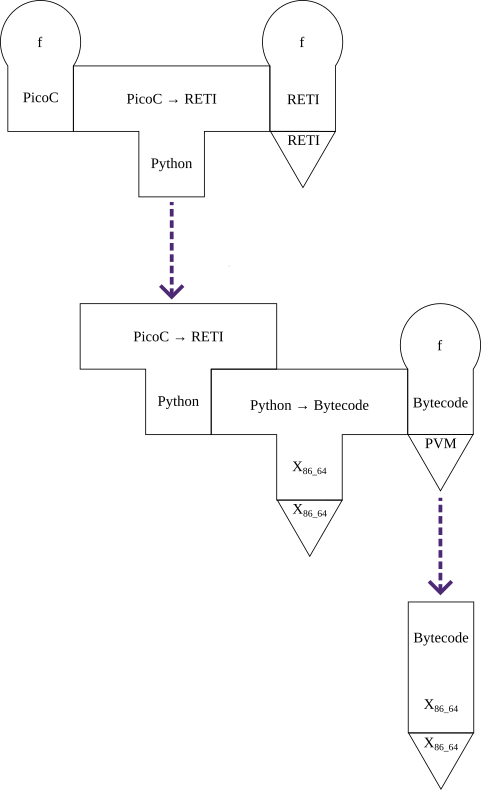
\includegraphics[width=0.5\linewidth]{./figures/summarized_cross_compiler.png}
  \caption{Cross-Compiler Kompiliervorgang ausgeschrieben}
\end{figure}

\begin{figure}[H]
  \centering
  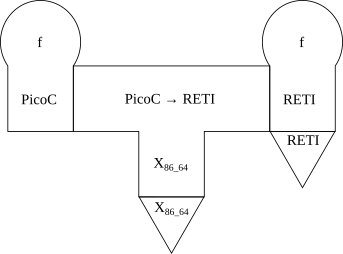
\includegraphics[width=0.33\linewidth]{./figures/compiliervorang_mit_machiene.png}
  \caption{Cross-Compiler Kompiliervorgang Kurzform}
\end{figure}

\begin{figure}[H]
  \centering
  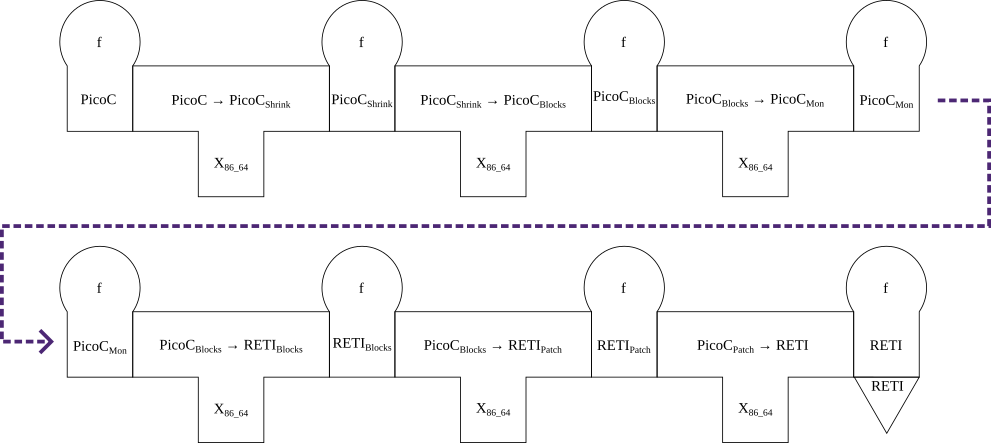
\includegraphics[width=\linewidth]{./figures/passes.png}
  \caption{Architektur mit allen Passes ausgeschrieben}
\end{figure}

\subsection{Passes}

\subsubsection{PicoC-Shrink Pass}
\label{picoc_shrink_pass}
% dieser Pass existiert nur wegen der Erweiterungen

\newlineparagraph{Codebeispiel}

\begin{code}
  \centering
  \numberedcodebox[minted language=c]{./code_examples/example_faculty_it.picoc}
  \caption{PicoC Code für Codebespiel}
  \label{code:picoc_code_für_codebeispiel}
\end{code}

\begin{code}
  \centering
  \numberedcodebox[minted language=text]{./code_examples/example_faculty_it.ast}
  \caption{Abstract Syntax Tree für Codebespiel}
  \label{code:abstract_syntax_tree_für_codebeispiel}
\end{code}

\begin{code}
  \centering
  \numberedcodebox[minted language=text]{./code_examples/example_faculty_it.picoc_shrink}
  \caption{PicoC Shrink Pass für Codebespiel}
  \label{code:picoc_shrink_pass_für_codebeispiel}
\end{code}

\subsubsection{PicoC-Blocks Pass}
\newlineparagraph{Abstrakte Syntax}
\begin{grammar}[Abstrakte Syntax für $L_{PicoC\_Blocks}$][H][gr:abstract_syntax_l_picoc_blocks]
  \toprule
  \firstcase{decl\_def}{FunDef(\langle datatype\rangle , Name(str),}{L\_Fun}
  & & \qquad $Alloc(Writeable(), \langle datatype\rangle , Name(str))*, \langle block\rangle *)$ & \\
  \midrule
  \firstcase{block}{Block(Name(str), \langle stmt\rangle *)}{L\_Blocks}
  \firstcase{stmt}{GoTo(Name(str)) \gralt NewStackframe(Name(), GoTo(str))}{}
  \otherform{RemoveStackframe() \gralt SetScope(Name(str))}{}
  \otherform{SingleLineComment(str, str)}{}
  \bottomrule
\end{grammar}

\newlineparagraph{Codebeispiel}

\begin{code}
  \centering
  \numberedcodebox[minted language=text]{./code_examples/example_faculty_it.picoc_blocks}
  \caption{PicoC-Blocks Pass für Codebespiel}
  \label{code:picoc_blocks_pass_für_codebeispiel}
\end{code}

\subsubsection{PicoC-Mon Pass}
\newlineparagraph{Abstrakte Syntax}
\begin{grammar}[Abstrakte Syntax für $L_{PicoC\_Mon}$][H][gr:abstract_syntax_l_picoc_mon]
  \toprule
  \firstcase{ref\_loc}{Stack(Num(str)) \gralt Global(Num(str))}{L\_Assign\_Alloc}
  \otherform{Stackframe(Num(str))}{}
  \firstcase{error\_data}{\langle exp\rangle  \gralt Pos(Num(str), Num(str))}{}
  \firstcase{exp}{Stack(Num(str)) \gralt Ref(\langle ref_loc\rangle , \langle datatype\rangle , \langle error_data\rangle )}{}
  \firstcase{stmt}{Exp(\langle exp\rangle )}{}
  \otherform{Assign(Alloc(Writeable(), StructSpec(Name(str)), Name(str)), }{}
  & & \qquad $Struct(Assign(Name(str), \langle exp\rangle )+, \langle datatype\rangle$ )) & \\
  \otherform{Assign(Alloc(Writeable(), ArrayDecl(Num(str)+, \langle datatype\rangle ),}{}
  & & \qquad $Name(str)), Array(\langle exp\rangle +, \langle datatype\rangle ))$ & \\
  \midrule
  \firstcase{symbol\_table}{SymbolTable(\langle symbol\rangle )}{L\_Symbol\_Table}
  \firstcase{symbol}{Symbol(\langle type_qual\rangle , \langle datatype\rangle , \langle name\rangle , \langle val\rangle , \langle pos\rangle , \langle size\rangle )}{}
  \firstcase{type\_qual}{Empty()}{}
  \firstcase{datatype}{BuiltIn() \gralt SelfDefined()}{}
  \firstcase{name}{Name(str)}{}
  \firstcase{val}{Num(str) \gralt Empty()}{}
  \firstcase{pos}{Pos(Num(str), Num(str)) \gralt Empty()}{}
  \firstcase{size}{Num(str) \gralt Empty()}{}
  \bottomrule
\end{grammar}

\begin{Definition}{Symboltabelle}{symboltabelle}
\end{Definition}

\newlineparagraph{Codebeispiel}

\begin{code}
  \centering
  \numberedcodebox[minted language=text]{./code_examples/example_faculty_it.picoc_mon}
  \caption{PicoC-Mon Pass für Codebespiel}
  \label{code:picoc_mon_pass_für_codebeispiel}
\end{code}

\subsubsection{RETI-Blocks Pass}
\newlineparagraph{Abstrakte Syntax}
\begin{grammar}[Abstrakte Syntax für $L_{RETI\_Blocks}$][H][gr:abstract_syntax_l_reti_blocks]
  \toprule
  \firstcase{program}{Program(Name(str), \langle block\rangle *)}{L\_Program}
  \midrule
  \firstcase{exp\_stmts}{GoTo(str)}{L\_Blocks}
  \firstcase{instrs\_before}{Num(str)}{}
  \firstcase{num\_instrs}{Num(str)}{}
  \firstcase{block}{Block(Name(str), \langle instr\rangle *, \langle instrs\_before\rangle , \langle num\_instrs\rangle )}{}
  \firstcase{instr}{GoTo(Name(str))}{}
  \bottomrule
\end{grammar}

\newlineparagraph{Codebeispiel}

\begin{code}
  \centering
  \numberedcodebox[minted language=text]{./code_examples/example_faculty_it.reti_blocks}
  \caption{RETI-Blocks Pass für Codebespiel}
  \label{code:reti_blocks_pass_für_codebeispiel}
\end{code}

\subsubsection{RETI-Patch Pass}
\newlineparagraph{Abstrakte Syntax}
\begin{grammar}[Abstrakte Syntax für $L_{RETI\_Patch}$][H][gr:abstract_syntax_l_reti_patch]
  \toprule
  \firstcase{stmt}{Exit(Num(str))}{}
  \bottomrule
\end{grammar}

\newlineparagraph{Codebeispiel}

\begin{code}
  \centering
  \numberedcodebox[minted language=text]{./code_examples/example_faculty_it.reti_patch}
  \caption{RETI-Patch Pass für Codebespiel}
  \label{code:reti_patch_pass_für_codebeispiel}
\end{code}

\subsubsection{RETI Pass}
\newlineparagraph{Konkrette und Abstrakte Syntax}

% dieser Pass entspricht Assembler bis auf die Sache mit binärer Repräsentation, was der PicoC-Compiler garnicht macht

\begin{grammar}[Konkrette Syntax für $L_{RETI\_Lex}$][H][gr:konkrette_syntax_l_reti_lexer]
\toprule
\firstcase{dig\_no\_0}{ \dq 1\dq \gralt \dq 2\dq \gralt \dq 3\dq \gralt \dq 4\dq \gralt \dq 5\dq \gralt \dq 6\dq}{L\_Program}
\otherform{\dq 7\dq \gralt \dq 8\dq \gralt \dq 9\dq}{}
\firstcase{dig\_with\_0}{ \dq 0\dq \gralt dig\_no\_0}{}
\firstcase{num}{ \dq 0\dq \gralt dig\_no\_0dig\_with\_0*\gralt \dq {-}\dq dig\_with\_0*}{}
\firstcase{letter}{ \dq a\dq ... \dq Z\dq }{}
\firstcase{name}{ letter(letter \mid  dig\_with\_0 \mid  \_)*}{}
\firstcase{reg}{ \dq ACC\dq \gralt \dq IN1\dq \gralt \dq IN2\dq \gralt \dq PC\dq \gralt \dq SP\dq}{}
\otherform{\dq BAF\dq \gralt \dq CS\dq \gralt \dq DS\dq}{}
\firstcase{arg}{ reg \gralt  num}{}
\firstcase{rel}{ \dq {==}\dq \gralt \dq {!=}\dq \gralt \dq {<}\dq \gralt \dq {<=}\dq\gralt \dq {>}\dq}{}
\otherform{\dq {>=}\dq \gralt \dq \_NOP\dq}{}
\bottomrule
\end{grammar}

\begin{grammar}[Konkrette Syntax für $L_{RETI\_Parse}$][H][gr:konkrette_syntax_l_reti_parser]
\toprule
\firstcase{instr}{\dq ADD\dq\enspace reg\enspace arg\gralt \dq ADDI\dq\enspace reg\enspace num\gralt \dq SUB\dq\enspace reg\enspace arg}{L\_Program}
\otherform{\dq SUBI\dq\enspace reg\enspace\enspace num\gralt \dq MULT\dq\enspace reg\enspace arg\gralt \dq MULTI\dq\enspace reg\enspace num}{}
\otherform{\dq DIV\dq\enspace reg\enspace arg\gralt \dq DIVI\dq\enspace reg\enspace num\gralt \dq MOD\dq\enspace reg\enspace arg}{}
\otherform{\dq MODI\dq\enspace reg\enspace num\gralt \dq OPLUS\dq\enspace reg\enspace arg\gralt \dq OPLUSI\dq\enspace reg\enspace num}{}
\otherform{\dq OR\dq\enspace reg\enspace arg\gralt \dq ORI\dq\enspace reg\enspace num}{}
\otherform{\dq AND\dq\enspace reg\enspace arg\gralt \dq ANDI\dq\enspace reg\enspace num}{}
\otherform{\dq LOAD\dq\enspace reg\enspace num\gralt \dq LOADIN\dq\enspace arg\enspace arg\enspace num}{}
\otherform{\dq LOADI\dq\enspace reg\enspace num}{}
\otherform{\dq STORE\dq\enspace reg\enspace num\gralt \dq STOREIN\dq\enspace arg\enspace arg num}{}
\otherform{\dq MOVE\dq\enspace reg\enspace reg}{}
\otherform{\dq JUMP\dq\enspace rel\enspace num\gralt INT\enspace num\gralt RTI}{}
\otherform{\dq CALL\dq\enspace \dq INPUT\dq\enspace  reg\gralt \dq CALL\dq\enspace \dq PRINT\dq\enspace reg}{}
\firstcase{program}{name\enspace (instr\dq ;\dq )*}{}
\bottomrule
\end{grammar}

% TODO: es braucht noch eine Konkrette Syntax dafür
\begin{grammar}[Abstrakte Syntax für $L_{RETI}$][H][gr:abstract_syntax_l_reti]
  \toprule
  \firstcase{reg}{ACC() \gralt IN1() \gralt IN2() \gralt PC() \gralt SP() \gralt BAF()}{L\_Program}
  \otherform{CS() \gralt DS()}{}
  \firstcase{arg}{Reg(\langle reg\rangle ) \gralt Num(str)}{}
  \firstcase{rel}{Eq() \gralt NEq() \gralt Lt() \gralt LtE() \gralt Gt() \gralt GtE()}{}
  \otherform{Always() \gralt NOp()}{}
  \firstcase{op}{Add() \gralt Addi() \gralt Sub() \gralt Subi() \gralt Mult()}{}
  \otherform{Multi() \gralt Div() \gralt Divi()}{}
  \otherform{Mod() \gralt Modi() \gralt Oplus() \gralt Oplusi() \gralt Or()}{}
  \otherform{Ori() \gralt And() \gralt Andi()}{}
  \otherform{Load() \gralt Loadin() \gralt Loadi()}{}
  \otherform{Store() \gralt Storein() \gralt Move()}{}
  \firstcase{instr}{Instr(\langle op\rangle , \langle arg\rangle +) \gralt Jump(\langle rel\rangle , Num(str)) \gralt Int(Num(str))}{}
  \otherform{RTI() \gralt Call(Name('print'), \langle reg\rangle ) \gralt Call(Name('input'), \langle reg\rangle )}{}
  \otherform{SingleLineComment(str, str)}{}
  \firstcase{program}{Program(Name(str), \langle instr\rangle *)}{}
  \bottomrule
\end{grammar}

\newlineparagraph{Codebeispiel}

\begin{code}
  \centering
  \numberedcodebox[minted language=text]{./code_examples/example_faculty_it.reti}
  \caption{RETI Pass für Codebespiel}
  \label{code:reti_pass_für_codebeispiel}
\end{code}

% TODO: zusammenfassendes Bild
         % ./content/Implementierung1.tex
  %!Tex Root = ../Main.tex
% ./Packete_und_Deklarationen.tex
% ./Titlepage.tex
% ./Motivation.tex
% ./Einführung.tex
% ./Implementierung1.tex
% ./Ergebnisse_und_Ausblick.tex

\subsection{Umsetzung von Pointern}
\subsubsection{Referenzierung}
Die \colorbold{Referenzierung} \verb|&var| wird im Folgenden anhand des Beispiels Code~\ref{code:picoc_code_für_pointer_referenzierung} erklärt.

\begin{code}
  \centering
  \numberedcodebox[minted language=c]{./code_examples/example_pntr_ref.picoc}
  \caption{PicoC Code für Pointer Referenzierung}
  \label{code:picoc_code_für_pointer_referenzierung}
\end{code}

Der Node \smalltt{Ref(Name('var')))} repräsentiert in der \colorbold{Abstrakten Syntax} in Code~\ref{code:abstract_syntax_tree_für_pointer_referenzierung} eine \colorbold{Referenzierung} \verb|&var|.

\begin{code}
  \centering
  \numberedcodebox[minted language=text]{./code_examples/example_pntr_ref.ast}
  \caption{Abstract Syntax Tree für Pointer Referenzierung}
  \label{code:abstract_syntax_tree_für_pointer_referenzierung}
\end{code}

Im \colorbold{PicoC-Mon Pass} in Code~\ref{code:picoc_mon_für_pointer_referenzierung} wird der Node \smalltt{Ref(Name('var')))} durch die Nodes \smalltt{Ref(GlobalRead(Num('0')))} und \smalltt{Assign(GlobalWrite(Num('1')), Tmp(Num('1')))} ersetzt. Im Fall, dass in \smalltt{Ref(exp))} das \smalltt{exp} vielleicht nicht direkt ein \smalltt{Name('var')} enthält und \smalltt{exp} vielleicht ein \smalltt{Subscr(Attr(Name('var')))} ist, sind noch weitere Anweisungen zwischen Zeile \smalltt{14} und  \smalltt{15} nötig, die sich in diesem Beispiel um das Übersetzen von \smalltt{Subscr(exp)} und \smalltt{Attr(exp)} kümmern. Die Vorgehen hierfür ist in Subkapitel~\ref{mittelteil_für_die_verschiedenen_derived_datatypes} erklärt.

\begin{code}
  \centering
  \numberedcodebox[minted language=text]{./code_examples/example_pntr_ref.picoc_mon}
  \caption{PicoC Mon Pass für Pointer Referenzierung}
  \label{code:picoc_mon_für_pointer_referenzierung}
\end{code}

Im \colorbold{PicoC-Blocks Pass} in Code~\ref{code:reti_blocks_für_pointer_referenzierung} wird der die Nodes \smalltt{}

\begin{code}
  \centering
  \numberedcodebox[minted language=text]{./code_examples/example_pntr_ref.reti_blocks}
  \caption{RETI Blocks Pass für Pointer Referenzierung}
  \label{code:reti_blocks_für_pointer_referenzierung}
\end{code}
% Initialisierung eines Pointers
\subsubsection{Pointer Dereferenzierung durch Zugriff auf Arrayindex ersetzen}
\begin{code}
  \centering
  \numberedcodebox[minted language=c]{./code_examples/example_pntr_deref.picoc}
  \caption{PicoC Code für Pointer Dereferenzierung}
  \label{code:picoc_code_für_pointer_dereferenzierung}
\end{code}

\begin{code}
  \centering
  \numberedcodebox[minted language=text]{./code_examples/example_pntr_deref.ast}
  \caption{Abstract Syntax Tree für Pointer Dereferenzierung}
  \label{code:abstract_syntax_tree_für_pointer_dereferenzierung}
\end{code}

\begin{code}
  \centering
  \numberedcodebox[minted language=text]{./code_examples/example_pntr_deref.picoc_shrink}
  \caption{PicoC Shrink Pass für Pointer Dereferenzierung}
  \label{code:picoc_shrink_für_pointer_dereferenzierung}
\end{code}

\subsection{Umsetzung von Arrays}
\subsubsection{Initialisierung von Arrays}
% Stack und Globale Statische Daten
\begin{code}
  \centering
  \numberedcodebox[minted language=c]{./code_examples/example_array_init.picoc}
  \caption{PicoC Code für Array Initialisierung}
  \label{code:picoc_code_für_array_initialisierung}
\end{code}

\begin{code}
  \centering
  \numberedcodebox[minted language=text]{./code_examples/example_array_init.ast}
  \caption{Abstract Syntax Tree für Array Initialisierung}
  \label{code:abstract_syntax_tree_für_array_initialisierung}
\end{code}

\begin{code}
  \centering
  \numberedcodebox[minted language=text]{./code_examples/example_array_init.st}
  \caption{Symboltabelle für Array Initialisierung}
  \label{code:symboltabelle_für_array_initialisierung}
\end{code}

\begin{code}
  \centering
  \numberedcodebox[minted language=text]{./code_examples/example_array_init.picoc_mon}
  \caption{PicoC Mon Pass für Array Initialisierung}
  \label{code:picoc_mon_für_array_initialisierung}
\end{code}

\begin{code}
  \centering
  \numberedcodebox[minted language=text]{./code_examples/example_array_init.reti_blocks}
  \caption{RETI Blocks Pass für Array Initialisierung}
  \label{code:reti_blocks_für_array_initialisierung}
\end{code}


% kleines Extra
\subsubsection{Zugriff auf Arrayindex}

Der Zugriff auf einen bestimmten  Index eines Arrays ist wie folgt umgesetzt:

\begin{code}
  \centering
  \numberedcodebox[minted language=c]{./code_examples/example_array_access.picoc}
  \caption{PicoC Code für Zugriff auf Arrayindex}
  \label{code:picoc_code_für_zugriff_auf_arrayindex}
\end{code}

\begin{code}
  \centering
  \numberedcodebox[minted language=text]{./code_examples/example_array_access.ast}
  \caption{Abstract Syntax Tree für Zugriff auf Arrayindex}
  \label{code:abstract_syntax_tree_für_zugriff_auf_arrayindex}
\end{code}

\begin{code}
  \centering
  \numberedcodebox[minted language=text]{./code_examples/example_array_access.picoc_mon}
  \caption{PicoC Mon Pass für Zugriff auf Arrayindex}
  \label{code:picoc_mon_für_zugriff_auf_arrayindex}
\end{code}

\begin{code}
  \centering
  \numberedcodebox[minted language=text]{./code_examples/example_array_access.reti_blocks}
  \caption{RETI Blocks Pass für Zugriff auf Arrayindex}
  \label{code:reti_blocks_für_zugriff_auf_arrayindex}
\end{code}

\subsubsection{Zuweisung an Arrayindex}
% Formel aus der Vorlesung, wo ist die hier?
\begin{code}
  \centering
  \numberedcodebox[minted language=c]{./code_examples/example_array_assignment.picoc}
  \caption{PicoC Code für Zuweisung an Arrayindex}
  \label{code:picoc_code_für_array_assignment}
\end{code}

\begin{code}
  \centering
  \numberedcodebox[minted language=text]{./code_examples/example_array_assignment.ast}
  \caption{Abstract Syntax Tree für Zuweisung an Arrayindex}
  \label{code:abstract_syntax_tree_für_array_assignment}
\end{code}

\begin{code}
  \centering
  \numberedcodebox[minted language=text]{./code_examples/example_array_assignment.picoc_mon}
  \caption{PicoC Mon Pass für Zuweisung an Arrayindex}
  \label{code:picoc_mon_für_array_assignment}
\end{code}

\begin{code}
  \centering
  \numberedcodebox[minted language=text]{./code_examples/example_array_assignment.reti_blocks}
  \caption{RETI Blocks Pass für Zuweisung an Arrayindex}
  \label{code:reti_blocks_für_array_assignment}
\end{code}

\subsection{Umsetzung von Structs}
\subsubsection{Deklaration von Structs}
\begin{code}
  \centering
  \numberedcodebox[minted language=c]{./code_examples/example_struct_decl.picoc}
  \caption{PicoC Code für Deklaration von Structs}
  \label{code:picoc_code_für_deklaration_von_structs}
\end{code}

\begin{code}
  \centering
  \numberedcodebox[minted language=text]{./code_examples/example_struct_decl.st}
  \caption{Symboltabelle für Deklaration von Structs}
  \label{code:symboltabelle_für_deklaration_von_structs}
\end{code}

\subsubsection{Initialisierung von Structs}
\begin{code}
  \centering
  \numberedcodebox[minted language=c]{./code_examples/example_struct_init.picoc}
  \caption{PicoC Code für Initialisierung von Structs}
  \label{code:picoc_code_für_initialisierung_von_structs}
\end{code}

\begin{code}
  \centering
  \numberedcodebox[minted language=text]{./code_examples/example_struct_init.ast}
  \caption{Abstract Syntax Tree für Initialisierung von Structs}
  \label{code:abstract_syntax_tree_für_initialisierung_von_structs}
\end{code}

\begin{code}
  \centering
  \numberedcodebox[minted language=text]{./code_examples/example_struct_init.st}
  \caption{Symboltabelle für Initialisierung von Structs}
  \label{code:symboltabelle_für_initialisierung_von_structs}
\end{code}

\begin{code}
  \centering
  \numberedcodebox[minted language=text]{./code_examples/example_struct_init.picoc_mon}
  \caption{PicoC Mon Pass für Initialisierung von Structs}
  \label{code:picoc_mon_pass_für_initialisierung_von_structs}
\end{code}

\begin{code}
  \centering
  \numberedcodebox[minted language=text]{./code_examples/example_struct_init.reti_blocks}
  \caption{RETI Blocks Pass für Initialisierung von Structs}
  \label{code:reti_blocks_pass_für_initialisierung_von_structs}
\end{code}

% Stack und Globale Statische Daten
\subsubsection{Zugriff auf Structattribut}
% Formel aus der Vorlesung, wo ist die hier?
\begin{code}
  \centering
  \numberedcodebox[minted language=c]{./code_examples/example_struct_attr_access.picoc}
  \caption{PicoC Code für Zugriff auf Structattribut}
  \label{code:picoc_code_für_zugriff_auf_structattribut}
\end{code}

\begin{code}
  \centering
  \numberedcodebox[minted language=text]{./code_examples/example_struct_attr_access.ast}
  \caption{Abstract Syntax Tree für Zugriff auf Structattribut}
  \label{code:abstract_syntax_tree_für_zugriff_auf_structattribut}
\end{code}

\begin{code}
  \centering
  \numberedcodebox[minted language=text]{./code_examples/example_struct_attr_access.picoc_mon}
  \caption{PicoC Mon Pass für Zugriff auf Structattribut}
  \label{code:picoc_mon_pass_für_zugriff_auf_structattribut}
\end{code}

\begin{code}
  \centering
  \numberedcodebox[minted language=text]{./code_examples/example_struct_attr_access.reti_blocks}
  \caption{RETI Blocks Pass für Zugriff auf Structattribut}
  \label{code:reti_blocks_pass_für_zugriff_auf_structattribut}
\end{code}

\subsubsection{Zuweisung an Structattribut}
\begin{code}
  \centering
  \numberedcodebox[minted language=c]{./code_examples/example_struct_attr_assignment.picoc}
  \caption{PicoC Code für Zuweisung an Structattribut}
  \label{code:picoc_code_für_zuweisung_an_structattribut}
\end{code}

\begin{code}
  \centering
  \numberedcodebox[minted language=text]{./code_examples/example_struct_attr_assignment.ast}
  \caption{Abstract Syntax Tree für Zuweisung an Structattribut}
  \label{code:abstract_syntax_tree_für_zuweisung_an_structattribut}
\end{code}

\begin{code}
  \centering
  \numberedcodebox[minted language=text]{./code_examples/example_struct_attr_assignment.picoc_mon}
  \caption{PicoC Mon Pass für Zuweisung an Structattribut}
  \label{code:picoc_mon_pass_für_zuweisung_an_structattribut}
\end{code}

\begin{code}
  \centering
  \numberedcodebox[minted language=text]{./code_examples/example_struct_attr_assignment.reti_blocks}
  \caption{RETI Blocks Pass für Zuweisung an Structattribut}
  \label{code:reti_blocks_pass_für_zuweisung_an_structattribut}
\end{code}

\subsection{Umsetzung der Derived Datatypes im Zusammenspiel}
\subsubsection{Einleitungsteil für Globale Statische Daten und Stackframe}
% Stack und Globale Statische Daten, unterschieldihe Berechnung der Adressen
% unterschiedliche Adressberechnung
\begin{code}
  \centering
  \numberedcodebox[minted language=c]{./code_examples/example_derived_dts_introduction_part.picoc}
  \caption{PicoC Code für den Einleitungsteil}
  \label{code:picoc_code_einleitungsteil}
\end{code}

% spezielles Vorgehen bei PntrDecl

\begin{code}
  \centering
  \numberedcodebox[minted language=text]{./code_examples/example_derived_dts_introduction_part.ast}
  \caption{Abstract Syntax Tree für den Einleitungsteil}
  \label{code:abstract_syntax_tree_einleitungsteil}
\end{code}

\begin{code}
  \centering
  \numberedcodebox[minted language=text]{./code_examples/example_derived_dts_introduction_part.picoc_mon}
  \caption{PicoC Mon Pass für den Einleitungsteil}
  \label{code:picoc_mon_pass_einleitungsteil}
\end{code}

\begin{code}
  \centering
  \numberedcodebox[minted language=text]{./code_examples/example_derived_dts_introduction_part.reti_blocks}
  \caption{RETI Blocks Pass für den Einleitungsteil}
  \label{code:reti_blocks_pass_einleitungsteil}
\end{code}

\subsubsection{Mittelteil für die verschiedenen Derived Datatypes}
\label{mittelteil_für_die_verschiedenen_derived_datatypes}

\begin{code}
  \centering
  \numberedcodebox[minted language=c]{./code_examples/example_derived_dts_main_part.picoc}
  \caption{PicoC Code für den Mittelteil}
  \label{code:picoc_code_mittelteil}
\end{code}

% spezielles Vorgehen bei PntrDecl

\begin{code}
  \centering
  \numberedcodebox[minted language=text]{./code_examples/example_derived_dts_main_part.ast}
  \caption{Abstract Syntax Tree für den Mittelteil}
  \label{code:abstract_syntax_tree_mittelteil}
\end{code}

\begin{code}
  \centering
  \numberedcodebox[minted language=text]{./code_examples/example_derived_dts_main_part.picoc_mon}
  \caption{PicoC Mon Pass für den Mittelteil}
  \label{code:picoc_mon_pass_mittelteil}
\end{code}

\begin{code}
  \centering
  \numberedcodebox[minted language=text]{./code_examples/example_derived_dts_main_part.reti_blocks}
  \caption{RETI Blocks Pass für den Mittelteil}
  \label{code:reti_blocks_pass_mittelteil}
\end{code}
% spezielles Vorgehen bei PntrDecl

\subsubsection{Schlussteil für die verschiedenen Derived Datatypes}
\begin{code}
  \centering
  \numberedcodebox[minted language=c]{./code_examples/example_derived_dts_final_part.picoc}
  \caption{PicoC Code für den Schlussteil}
  \label{code:picoc_code_schlussteil}
\end{code}

\begin{code}
  \centering
  \numberedcodebox[minted language=text]{./code_examples/example_derived_dts_final_part.ast}
  \caption{Abstract Syntax Tree für den Schlussteil}
  \label{code:abstract_syntax_tree_schlussteil}
\end{code}

\begin{code}
  \centering
  \numberedcodebox[minted language=text]{./code_examples/example_derived_dts_final_part.picoc_mon}
  \caption{PicoC Mon Pass für den Schlussteil}
  \label{code:picoc_mon_pass_schlussteil}
\end{code}

\begin{code}
  \centering
  \numberedcodebox[minted language=text]{./code_examples/example_derived_dts_final_part.reti_blocks}
  \caption{RETI Blocks Pass für den Schlussteil}
  \label{code:reti_blocks_pass_schlussteil}
\end{code}

% Umgang, wenn Datentyp abrubt aufhört am Ende

\subsection{Umsetzung von Funktionen}
\subsubsection{Funktionen auflösen zu RETI Code}
\begin{code}
  \centering
  \numberedcodebox[minted language=c]{./code_examples/example_3_funs.picoc}
  \caption{PicoC Code für 3 Funktionen}
  \label{code:picoc_code_für_3_Funktionen}
\end{code}

\begin{code}
  \centering
  \numberedcodebox[minted language=text]{./code_examples/example_3_funs.ast}
  \caption{Abstract Syntax Tree für 3 Funktionen}
  \label{code:abstract_syntax_tree_für_3_Funktionen}
\end{code}

\begin{code}
  \centering
  \numberedcodebox[minted language=text]{./code_examples/example_3_funs.picoc_blocks}
  \caption{PicoC Blocks Pass für 3 Funktionen}
  \label{code:picoc_blocks_pass_für_3_Funktionen}
\end{code}

\begin{code}
  \centering
  \numberedcodebox[minted language=text]{./code_examples/example_3_funs.picoc_mon}
  \caption{PicoC Mon Pass für 3 Funktionen}
  \label{code:picoc_mon_pass_für_3_Funktionen}
\end{code}

\begin{code}
  \centering
  \numberedcodebox[minted language=text]{./code_examples/example_3_funs.reti_blocks}
  \caption{RETI Blocks Pass für 3 Funktionen}
  \label{code:reti_blocks_pass_für_3_Funktionen}
\end{code}

% einfügen unsichtbarer Returns bei void
\newlineparagraph{Sprung zur Main Funktion}

\begin{code}
  \centering
  \numberedcodebox[minted language=c]{./code_examples/example_3_funs_main.picoc}
  \caption{PicoC Code für Funktionen, wobei die main Funktion nicht die erste Funktion ist}
  \label{code:picoc_code_für_funktionen_wobei_die_main_funktion_nicht_die_erste_Funktion_ist}
\end{code}

\begin{code}
  \centering
  \numberedcodebox[minted language=text]{./code_examples/example_3_funs_main.picoc_mon}
  \caption{PicoC Mon Pass für Funktionen, wobei die main Funktion nicht die erste Funktion ist}
  \label{code:picoc_mon_pass_für_funktionen_wobei_die_main_funktion_nicht_die_erste_Funktion_ist}
\end{code}

\begin{code}
  \centering
  \numberedcodebox[minted language=text]{./code_examples/example_3_funs_main.reti_blocks}
  \caption{PicoC Blocks Pass für Funktionen, wobei die main Funktion nicht die erste Funktion ist}
  \label{code:picoc_blocks_pass_für_funktionen_wobei_die_main_funktion_nicht_die_erste_Funktion_ist}
\end{code}

\begin{code}
  \centering
  \numberedcodebox[minted language=text]{./code_examples/example_3_funs_main.reti_patch}
  \caption{PicoC Patch Pass für Funktionen, wobei die main Funktion nicht die erste Funktion ist}
  \label{code:picoc_patch_pass_für_funktionen_wobei_die_main_funktion_nicht_die_erste_Funktion_ist}
\end{code}

\subsubsection{Funktionsdeklaration und -definition}
\begin{code}
  \centering
  \numberedcodebox[minted language=c]{./code_examples/example_3_funs_fun_decl.picoc}
  \caption{PicoC Code für Funktionen, wobei eine Funktion vorher deklariert werden muss}
  \label{code:picoc_code_für_funktionen_picoc_code_für_funktionen_wobei_eine_funktion_vorher_deklariert_werden_muss}
\end{code}

\begin{code}
  \centering
  \numberedcodebox[minted language=text]{./code_examples/example_3_funs_fun_decl.st}
  \caption{Symboltabelle für Funktionen, wobei eine Funktion vorher deklariert werden muss}
  \label{code:symboltabelle_für_funktionen_picoc_code_für_funktionen_wobei_eine_funktion_vorher_deklariert_werden_muss}
\end{code}

% Allocation von Variablen
% Stack und Globale Statische Daten
% die Sache mit Assign(Tmp, Global) und Assign(Global, Tmp)
% erwähnen, das Main Funktion keinen Stackframe hat
% zählen der Größe der lokalen Daten und Parameter
% TODO: Signatur zu Parameter umbenennen
\subsubsection{Funktionsaufruf}

\newlineparagraph{Ohne Rückgabewert}

% Unsichtbares return
\begin{code}
  \centering
  \numberedcodebox[minted language=c]{./code_examples/example_fun_call_no_return_value.picoc}
  \caption{PicoC Code für Funktionsaufruf ohne Rückgabewert}
  \label{code:picoc_code_für_funktionsaufruf_ohne_rückgabewert}
\end{code}

\begin{code}
  \centering
  \numberedcodebox[minted language=text]{./code_examples/example_fun_call_no_return_value.picoc_mon}
  \caption{PicoC Mon Pass für Funktionsaufruf ohne Rückgabewert}
  \label{code:picoc_mon_pass_für_funktionsaufruf_ohne_rückgabewert}
\end{code}

\begin{code}
  \centering
  \numberedcodebox[minted language=text]{./code_examples/example_fun_call_no_return_value.reti_blocks}
  \caption{RETI Blocks Pass für Funktionsaufruf ohne Rückgabewert}
  \label{code:reti_blocks_pass_für_funktionsaufruf_ohne_rückgabewert}
\end{code}

\begin{code}
  \centering
  \numberedcodebox[minted language=text]{./code_examples/example_fun_call_no_return_value.reti}
  \caption{RETI Pass für Funktionsaufruf ohne Rückgabewert}
  \label{code:reti_pass_für_funktionsaufruf_ohne_rückgabewert}
\end{code}

\newlineparagraph{Mit Rückgabewert}

\begin{code}
  \centering
  \numberedcodebox[minted language=c]{./code_examples/example_fun_call_with_return_value.picoc}
  \caption{PicoC Code für Funktionsaufruf mit Rückgabewert}
  \label{code:picoc_code_für_funktionsaufruf_mit_rückgabewert}
\end{code}

\begin{code}
  \centering
  \numberedcodebox[minted language=text]{./code_examples/example_fun_call_with_return_value.picoc_mon}
  \caption{PicoC Mon Pass für Funktionsaufruf mit Rückgabewert}
  \label{code:picoc_mon_pass_für_funktionsaufruf_mit_rückgabewert}
\end{code}

\begin{code}
  \centering
  \numberedcodebox[minted language=text]{./code_examples/example_fun_call_with_return_value.reti_blocks}
  \caption{RETI Blocks Pass für Funktionsaufruf mit Rückgabewert}
  \label{code:reti_blocks_pass_für_funktionsaufruf_mit_rückgabewert}
\end{code}

\begin{code}
  \centering
  \numberedcodebox[minted language=text]{./code_examples/example_fun_call_with_return_value.reti}
  \caption{RETI Pass für Funktionsaufruf mit Rückgabewert}
  \label{code:reti_pass_für_funktionsaufruf_mit_rückgabewert}
\end{code}

\newlineparagraph{Umsetzung von Call by Sharing für Arrays}

\begin{code}
  \centering
  \numberedcodebox[minted language=c, minted options={highlightlines={1,7}}]{./code_examples/example_fun_call_by_sharing_array.picoc}
  \caption{PicoC Code für Call by Sharing für Arrays}
  \label{code:picoc_code_für_call_by_sharing_für_arrays}
\end{code}

\begin{code}
  \centering
  \numberedcodebox[minted language=text, minted options={highlightlines={15-20}}]{./code_examples/example_fun_call_by_sharing_array.picoc_mon}
  \caption{PicoC Mon Pass für Call by Sharing für Arrays}
  \label{code:picoc_mon_pass_für_call_by_sharing_für_arrays}
\end{code}


% https://tex.stackexchange.com/questions/298383/how-to-highlight-color-draw-attention-to-a-particular-snippet-in-minted/498614#498614
\begin{code}
  \centering
  \numberedcodebox[minted language=text, minted options={highlightlines={15,24}}]{./code_examples/example_fun_call_by_sharing_array.st}
  \caption{Symboltabelle für Call by Sharing für Arrays}
  \label{code:symboltabelle_für_call_by_sharing_für_arrays}
\end{code}

\begin{code}
  \centering
  \numberedcodebox[minted language=text, minted options={highlightlines={13-20}}]{./code_examples/example_fun_call_by_sharing_array.reti_blocks}
  \caption{RETI Block Pass für Call by Sharing für Arrays}
  \label{code:reti_blocks_pass_für_call_by_sharing_für_arrays}
\end{code}

% die Sache mit dem erstetzen von ArryDecl durch PntrDecl

\newlineparagraph{Umsetzung von Call by Value für Structs}

\begin{code}
  \centering
  \numberedcodebox[minted language=c, minted options={highlightlines={8}}]{./code_examples/example_fun_call_by_value_struct.picoc}
  \caption{PicoC Code für Call by Value für Structs}
  \label{code:picoc_code_für_call_by_value_für_structs}
\end{code}

% argmode für Struct Call by Value

\begin{code}
  \centering
  \numberedcodebox[minted language=text, minted options={highlightlines={15-19}}]{./code_examples/example_fun_call_by_value_struct.picoc_mon}
  \caption{PicoC Mon Pass für Call by Value für Structs}
  \label{code:picoc_mon_pass_für_call_by_value_for_structs}
\end{code}

% hier könnte man anmerken, dass die Adressen unterschiedlich berechnet werden für Stack und Globale...

\begin{code}
  \centering
  \numberedcodebox[minted language=text, minted options={highlightlines={13-19}}]{./code_examples/example_fun_call_by_value_struct.reti_blocks}
  \caption{RETI Block Pass für Call by Value für Structs}
  \label{code:reti_blocks_pass_für_call_by_value_for_structs}
\end{code}

% Struct wird wirklich kopiert durch speziellen Argmode

\subsection{Umsetzung kleinerer Details}
% langen Sprüngen, großen Konstanten, Division durch 0
\section{Fehlermeldungen}
\subsection{Error Handler}
\subsection{Arten von Fehlermeldungen}
\subsubsection{Syntaxfehler}
\subsubsection{Laufzeitfehler}
% Fehlermeldung ist, wenn der Lexer (partielle Funktion) oder Parser nicht matcht
% Token und Nodes enthalten Position, im Transformer wird die Position von den Token auf die Nodes übertragen und auch die Symboltabelle speichert Position
         % ./content/Implementierung2.tex
  %!Tex Root = ../Main.tex
% ./Packete_und_Deklarationen.tex
\chapter{Ergebnisse und Ausblick}
\label{ch:ergebnisse_und_ausblick}

  % https://www.overleaf.com/learn/latex/Counters
\counterwithin{defcounter}{chapter}

\section{Funktionsumfang}
\section{Qualitätssicherung}
% GCC + Execution entspricht einem einzigen großen Interpreter und beweist somit den linke Edge in 2.1
\label{sec:qualitätssicherung}
% RETI-Interpreter erwähnen
% TODO: zusammenfassendes Bild
\section{Kommentierter Kompiliervorgang}
\section{Erweiterungsideen}
Wenn eines Tages eine \colorbold{RETI-CPU} auf einem \colorbold{FPGA} implementiert werden sollte, sodass ein \colorbold{provisorisches Betriebssystem} darauf laufen könnte, dann wäre der nächste Schritt einen \colorbold{Self-Compiling Compiler} $C_{PicoC}^{PicoC}$ (Defintion~\ref{def:self_compiling_compiler}) zu schreiben, der selbst in der Programmiersprache $L_{PicoC}$ geschrieben ist und sich selbst kompilieren kann. Je nach Implementierungsart dieses \colorbold{Self-compiling Compiler} kann dadurch \colorbold{Unabhängigkeit} von der Programmiersprache \colorbold{Python}, in der der momentane Compiler $C_{PicoC}$ für $L_{PicoC}$ momentan implementiert ist und Unabhängigkeit von einer anderen Maschiene, die bisher immer für das \colorbold{Cross-Compiling} notwendig war erreicht werden.

\begin{Definition}{Self-compiling Compiler}{self_compiling_compiler}
  Compiler $C_w^w$, der in der Sprache $L_w$ \colorbold{geschrieben} ist, die er \colorbold{selbst} kompiliert. Also ein Compiler, der sich \colorbold{selbst} kompilieren könnte.
\end{Definition}

Will man nun für eine Maschiene $M_{RETI}$, auf der bisher keine anderen Programmiersprachen mittels \colorbold{Bootstrapping} (Definition~\ref{def:bootstrapping}) zum laufen gebracht wurden, den gerade beschriebenen \colorbold{Self-compiling Compiler} $C_{PicoC}^{PicoC}$ implementieren und hat bereits den gesamtem \colorbold{Self-compiling Compiler} $C_{PicoC}^{PicoC}$ in der Sprache  $L_{PicoC}$ geschrieben, so stösst man auf ein Problem, dass auf das \colorbold{Henne-Ei-Problem}\footnote{Beschreibt die Situation, wenn ein System sich selbst als \colorbold{Abhängigkeit} hat, damit es überhaupt einen \colorbold{Anfang} für dieses System geben kann. Dafür steht das Problem mit der \colorbold{Henne} und dem \colorbold{Ei} sinnbildlich, da hier die Frage ist, wie das ganze seinen Anfang genommen hat, da beides \colorbold{zirkular} voneinander abhängt.} reduziert werden kann. Man bräuchte, um den \colorbold{Self-compiling Compiler} $C_{PicoC}^{PicoC}$ auf der \colorbold{Maschiene} $M_{RETI}$ zu kompilieren bereits einen kompilierten \colorbold{Self-compiling Compiler} $C_{PicoC}^{PicoC}$, der mit der Maschienensprache \colorbold{RETI} läuft. Es liegt eine \colorbold{zirkulare Abhängigkeit} vor, die man nur auflösen kann, indem eine \colorbold{externe Entität} zur Hilfe nimmt.

Da man den gesamten \colorbold{Self-compiling Compiler} $C_{PicoC}^{PicoC}$ nicht selbst komplett in der Maschienensprache \colorbold{RETI} schreiben will, wäre eine Möglichkeit, dass man den \colorbold{Cross-Compiler} $C_{PicoC}^{Python}$, den man bereits in der Programmiersprache \colorbold{Python} implementiert hat, der in diesem Fall die \colorbold{externe Entität} darstellt, auf einer anderen Maschiene $M$ dafür nutzt, damit dieser den \colorbold{Self-compiling Compiler} $C_{PicoC}^{PicoC}$ für die Maschiene $M_{RETI}$ kompiliert bzw. \colorbold{bootstraped} und man den kompilierten \colorbold{RETI-Maschiendencode} dann einfach auf die Maschiene $M_{RETI}$ kopiert.\footnote{Im Fall, dass auf der Maschiene $M_{RETI}$ die Programmiersprache $L_{Python}$ bereits mittels \colorbold{Bootstrapping} zum Laufen gebracht wurde, könnte der \colorbold{Self-compiling Compiler} $C_{PicoC}^{PicoC}$ auch mithife des \colorbold{Cross-Compilers} $C_{PicoC}^{Python}$ als \colorbold{externe Entität} und der Programmiersprache \colorbold{Python} auf der Maschiene $M_{RETI}$ selbst kompiliert werden.}

Aufbauend auf dem \colorbold{Self-compiling Compiler} $C_{PicoC}^{PicoC}$, der einen \colorbold{minimalen Compiler} (Definition~\ref{def:minimaler_compiler}) für eine Teilmenge der \colorbold{Programmiersprache} C bzw. $L_C$ darstellt, könnte man auch noch die komplette Sprache $L_C$ für die Maschiene $M_{RETI}$ mittels \colorbold{Bootstrapping} (Defintion~\nameref{par:bootstrapping}) implementieren.\footnote{Natürlich könnte man aber auch einfach den \colorbold{Cross-Compiler} $C_{PicoC}^{Python}$ um weitere Funktionalitäten von $L_C$ erweitern, hat dann aber weiterhin eine \colorbold{Abhängigkeit} von der Programmiersprache \colorbold{Python}.}

\begin{Special_Paragraph}
  Einen ersten \colorbold{minimalen Compiler} $C_{2\_min}$ für eine Maschiene $M_2$, kann man entweder mittels eines \colorbold{externen} \colorbold{Bootstrap Compilers} (Definition~\ref{def:bootstrap_compiler}) $C_o$ kompilieren\footnote{In diesem Fall, dem \colorbold{Cross-Compiler} $C_{PicoC}^{Python}$.} oder man schreibt in direkt in der \colorbold{Maschienensprache} $B_2$ bzw. wenn ein \colorbold{Assembler} vorhanden ist, in der \colorbold{Assemblesprache} $A_2$.

  Die letzte Option wäre allerdings nur beim allerersten Compiler $C_{first}$ für eine allererste \colorbold{abstraktere Programmiersprache} $L_{first}$ mit Schleifen, Verzweigungen usw. notwendig gewesen. Ansonsten hätte man immer eine Kette, die beim allersten Compiler $C_{first}$ anfängt fortführen können, in der ein Compiler einen anderen Compiler kompiliert bzw. einen ersten minimalen Compiler kompiliert und dieser minimale Compiler dann eine umfangreichere Version von sich kompiliert usw.

  Bei einem \colorbold{Bootstrap Compiler} handelt es sich um einen Compiler in einer anderen Programiersprache $L_o$, der entweder ein \colorbold{Cross-Compiler} auf einer anderen Maschiene $M_1$ ist oder lokal auf der Maschiene $M_2$ läuft.
\end{Special_Paragraph}

\begin{Definition}{Minimaler Compiler}{minimaler_compiler}
  Compiler $C_{w\_min}$, der nur die \colorbold{notwendigsten Funktionalitäten} einer Sprache $L_w$, wie \colorbold{Schleifen},  \colorbold{Verzweigungen} kompiliert, die für die Implementierung eines \colorbold{Self-compiling Compilers} $C_{w}^{w}$ oder einer \colorbold{ersten Version} $C_{w_i}^{w_i}$ des Self-compiling Compilers $C_w^w$ für diese Sprache $L_w$ wichtig sind.\footnote{Den \colorbold{PicoC-Compiler} könnte man auch als einen \colorbold{minimalen Compiler} ansehen}
\end{Definition}{}{}

\begin{Definition}{Boostrap Compiler}{bootstrap_compiler}
  Compiler $C_o$, der es ermöglicht einen \colorbold{Self-compiling Compiler} $C_w^w$ zu \colorbold{boostrapen}, indem der Self-compiling Compiler $C_w^w$ in der Sprache $L_o$ des Bootstrap Compilers $C_o$ \colorbold{geschrieben} und mit diesem \colorbold{kompiliert} wird. Dies ermöglicht es die \colorbold{zirkulare Abhängikeit}, dass initial ein \colorbold{Self-compiling Compiler} bereits kompiliert vorliegen müsste, um sich selbst kompilieren zu können, zu brechen.

  \setcounter{defcounter}{\value{\tcbcounter}}
  \stepcounter{defcounter}
\end{Definition}

eben in einer \colorbold{Programmiersprache} $L_o$ implementiert hat, in der \colorbold{Wunschsprache} $L_w$ selbst implementieren und dann mit dem \colorbold{minamlen Compiler} für ebendiese Wunschsprache selbst kompilieren. Was man als Output bekommt ist ein \colorbold{minimmaler Compiler}, der aber auf der \colorbold{Zielmaschine} läuft und die \colorbold{Wunschsprache} in die \colorbold{Maschienensprache} der Zielmaschine kompiliert.

Aufbauend auf diesem \colorbold{minimalen Compiler}, der auf der \colorbold{Zielmaschine} läuft, kann man nun auf der Zielmaschine selbst \colorbold{iterativ} den minimalen Compiler schrittweise zu einem umfangreicheren Compiler, der mehr Funktionalitäten unterstützt weiterentwickeln und braucht die ursprüngliche Maschine, auf dem man die allererste Version des minimalen Compilers implementiert hat nicht mehr. Dieses Vorgehen wird auch als \colorbold{Bootstrapping} (Definition~\ref{def:bootstrapping}) bezeichnet.\footnote{Der Begriff hat seinen Ursprung in der englischen \colorbold{Redewendung} \glqq pulling yourself up by your own bootstraps\grqq, was im deutschen ungefähr der aus den \colorbold{Lügengeschichten des Freiherrn von Münchhausen} bekannten Redewendung \glqq sich am eigenen Schopf aus dem Sumpf ziehen\grqq entspricht.}

\begin{Definition}{Bootstrapping}{bootstrapping}
  Wenn man einen \colorbold{Self-compiling Compiler} $C_{w}^{w}$ einer Wunschsprache $L_w$ auf einer \colorbold{Zielmaschine} $M$ zum laufen bringt\footnote{Z.B. mithilfe eines \colorbold{Bootstrap Compilers}.}\footnote{Hat man einmal einen solchen \colorbold{Self-compiling Compiler} $C_{w}^{w}$ auf der Maschiene $M$ zum laufen gebracht, so kann man den Compiler auf der Maschiene $M$ weiterentwicklern, ohne von externen Entitäten, wie einer bestimmten Sprache $L_o$, in der der Compiler oder eine frühere Version des Compilers ursprünglich geschrieben war abhängig zu sein.}\footnote{Einen Compiler in der Sprache zu schreiben, die er selbst kompiliert und diesen Compiler dann sich selbst kompilieren zu lassen kann eine gute \colorbold{Probe aufs Exempel} darstellen, dass der Compiler auch wirklich funktioniert.}. Dabei ist die Art von \colorbold{Bootstrapping} in \nameref{par:bootstrapping} nochmal gesondert hervorzuheben:

  % https://tex.stackexchange.com/questions/7627/how-to-reference-paragraph
  \titleformat{\paragraph}[runin]{\normalfont\normalsize\bfseries}{}{0mm}{}[:]

  % https://tex.stackexchange.com/questions/7627/how-to-reference-paragraph
  \paragraph{\thedefcounter{.1}}\label{par:bootstrapping}\hspace{-0.25cm}
  Wenn man die \colorbold{aktuelle Version} eines \colorbold{Self-compiling Compilers} $C_{w_i}^{w_i}$ der Wunschsprache $L_{w_i}$ mithilfe von \colorbold{früheren Versionen} seiner selbst kompiliert. Man schreibt also z.B. die aktuelle Version des Self-compiling Compilers in der Sprache $L_{w_{i-1}}$, welche von der früheren Version des Compilers, dem Self-compiling Compiler $C_{w_{i-1}}^{w_{i-1}}$ kompiliert wird und schafft es so \colorbold{iterativ} immer umfangreichere Compiler zu bauen.\footnote{Compiler}\footnote{Es ist hierbei theoretisch nicht notwendig den \colorbold{letzten} Self-compiling Compiler $C_{w_{i-1}}^{w_{i-1}}$ für das Kompilieren des \colorbold{neuen} Self-compiling Compilers $C_{w_i}^{w_i}$ zu verwenden, wenn z.B. der \colorbold{Self-compiling Compiler} $C_{w_{i-3}}^{w_{i-3}}$ auch bereits alle Funktionalitäten, die beim Schreiben des \colorbold{Self-compiling Compilers} $C_w^w$ verwendet werden kompilieren kann.}\footnote{Der Begriff ist sinnverwandt mit dem \colorbold{Booten} eines Computers, wo die wichtigste Software, der \colorbold{Kernel} zuerst in den Speicher geladen wird und darauf aufbauend von diesem dann das Betriebssysteme, welches bei Bedarf dann \colorbold{Systemsoftware}, Software, die das Ausführen von Anwendungssoftware ermöglicht oder unterstützt, wie z.B. Treiber. und \colorbold{Anwendungssoftware}, Software, deren Anwendung darin besteht, dass sie dem Benutzer unmittelbar eine Dienstleistung zur Verfügung stellt, lädt.}\footcite{earley_formalism_1970}
\end{Definition}

\begin{Special_Paragraph}
Auch wenn ein \colorbold{Self-compiling Compiler} $C_{w_i}^{w_i}$ in der Subdefinition~\nameref{par:bootstrapping} selbst in einer früheren Version $L_{w_{i-1}}$ der Programmiersprache $L_{w_i}$, geschrieben wird, wird dieser nicht mit $C_{w_i}^{w_{i-1}}$ bezeichnet, sondern mit $C_{w_i}}^{w_i}$, da es bei \colorbold{Self-compiling Compilern} darum geht, dass diese zwar in der Subdefinition~\nameref{par:bootstrapping} eine frühere Version $C_{w_{i-1}}^{w_{i-1}}$ nutzen, um sich selbst kompiliert zu lassen, aber sie auch in der Lage sind sich selber zu kompilieren.
\end{Special_Paragraph}
 % ./content/Ergebnisse_und_Ausblick.tex

  \appendix
  %!Tex Root = ../Main.tex
% ./Packete_und_Deklarationen.tex

% \changelocaltocdepth{0}

\chapter*{Appendix}
\label{appendix}
\addcontentsline{toc}{chapter}{Appendix}

\section*{Konkrette und Abstrakte Syntax}
\section*{Bedienungsanleitungen}
\subsection*{PicoC-Compiler}
\subsection*{Showmode}
\subsection*{Entwicklertools}
                % ./content/Appendix.tex
  %!Tex Root=../Main.tex
% ./Packete_und_Deklarationen.tex
\chapter{Danksagungen}
            % ./content/Danksagungen.tex

  \printbibheading
  % \printbibliography[type=book,heading=subbibliography,title={Bücher}]
  % \printbibliography[type=article,heading=subbibliography,title={Artikel}]
  \printbibliography[type=online,heading=subbibliography,title={Online}]
  \printbibliography[type=book,heading=subbibliography,title={Bücher}]
  \printbibliography[type=article,heading=subbibliography,title={Artikel}]
  \printbibliography[type=unpublished,heading=subbibliography,title={Vorlesungen}]
  \printbibliography[nottype=book, nottype=article, nottype=online, nottype=unpublished,heading=subbibliography,title={Sonstige Quellen}]
  % ./Library.bib
\end{document}
